% Options for packages loaded elsewhere
\PassOptionsToPackage{unicode}{hyperref}
\PassOptionsToPackage{hyphens}{url}
\PassOptionsToPackage{dvipsnames,svgnames*,x11names*}{xcolor}
%
\documentclass[
  11pt,
]{article}
\usepackage{lmodern}
\usepackage{amssymb,amsmath}
\usepackage{ifxetex,ifluatex}
\ifnum 0\ifxetex 1\fi\ifluatex 1\fi=0 % if pdftex
  \usepackage[T1]{fontenc}
  \usepackage[utf8]{inputenc}
  \usepackage{textcomp} % provide euro and other symbols
\else % if luatex or xetex
  \usepackage{unicode-math}
  \defaultfontfeatures{Scale=MatchLowercase}
  \defaultfontfeatures[\rmfamily]{Ligatures=TeX,Scale=1}
  \setmainfont[Path=/usr/share/fonts/truetype/dejavu/]{DejaVuSerif.ttf}
  \setmonofont[Path=/usr/share/fonts/truetype/dejavu/]{DejaVuSansMono.ttf}
\fi
% Use upquote if available, for straight quotes in verbatim environments
\IfFileExists{upquote.sty}{\usepackage{upquote}}{}
\IfFileExists{microtype.sty}{% use microtype if available
  \usepackage[]{microtype}
  \UseMicrotypeSet[protrusion]{basicmath} % disable protrusion for tt fonts
}{}
\makeatletter
\@ifundefined{KOMAClassName}{% if non-KOMA class
  \IfFileExists{parskip.sty}{%
    \usepackage{parskip}
  }{% else
    \setlength{\parindent}{0pt}
    \setlength{\parskip}{6pt plus 2pt minus 1pt}}
}{% if KOMA class
  \KOMAoptions{parskip=half}}
\makeatother
\usepackage{xcolor}
\IfFileExists{xurl.sty}{\usepackage{xurl}}{} % add URL line breaks if available
\IfFileExists{bookmark.sty}{\usepackage{bookmark}}{\usepackage{hyperref}}
\hypersetup{
  pdftitle={A Continuous-Encoding Breakthrough for Multi-Objective Torso Decomposition},
  pdfauthor={Adrian Ymeri --- University of Prishtina · SpOC-3 Torso Decompositions},
  colorlinks=true,
  linkcolor=blue,
  filecolor=Maroon,
  citecolor=Blue,
  urlcolor=blue,
  pdfcreator={LaTeX via pandoc}}
\urlstyle{same} % disable monospaced font for URLs
\usepackage[margin=1in]{geometry}
\usepackage{color}
\usepackage{fancyvrb}
\newcommand{\VerbBar}{|}
\newcommand{\VERB}{\Verb[commandchars=\\\{\}]}
\DefineVerbatimEnvironment{Highlighting}{Verbatim}{commandchars=\\\{\}}
% Add ',fontsize=\small' for more characters per line
\newenvironment{Shaded}{}{}
\newcommand{\AlertTok}[1]{\textcolor[rgb]{1.00,0.00,0.00}{\textbf{#1}}}
\newcommand{\AnnotationTok}[1]{\textcolor[rgb]{0.38,0.63,0.69}{\textbf{\textit{#1}}}}
\newcommand{\AttributeTok}[1]{\textcolor[rgb]{0.49,0.56,0.16}{#1}}
\newcommand{\BaseNTok}[1]{\textcolor[rgb]{0.25,0.63,0.44}{#1}}
\newcommand{\BuiltInTok}[1]{#1}
\newcommand{\CharTok}[1]{\textcolor[rgb]{0.25,0.44,0.63}{#1}}
\newcommand{\CommentTok}[1]{\textcolor[rgb]{0.38,0.63,0.69}{\textit{#1}}}
\newcommand{\CommentVarTok}[1]{\textcolor[rgb]{0.38,0.63,0.69}{\textbf{\textit{#1}}}}
\newcommand{\ConstantTok}[1]{\textcolor[rgb]{0.53,0.00,0.00}{#1}}
\newcommand{\ControlFlowTok}[1]{\textcolor[rgb]{0.00,0.44,0.13}{\textbf{#1}}}
\newcommand{\DataTypeTok}[1]{\textcolor[rgb]{0.56,0.13,0.00}{#1}}
\newcommand{\DecValTok}[1]{\textcolor[rgb]{0.25,0.63,0.44}{#1}}
\newcommand{\DocumentationTok}[1]{\textcolor[rgb]{0.73,0.13,0.13}{\textit{#1}}}
\newcommand{\ErrorTok}[1]{\textcolor[rgb]{1.00,0.00,0.00}{\textbf{#1}}}
\newcommand{\ExtensionTok}[1]{#1}
\newcommand{\FloatTok}[1]{\textcolor[rgb]{0.25,0.63,0.44}{#1}}
\newcommand{\FunctionTok}[1]{\textcolor[rgb]{0.02,0.16,0.49}{#1}}
\newcommand{\ImportTok}[1]{#1}
\newcommand{\InformationTok}[1]{\textcolor[rgb]{0.38,0.63,0.69}{\textbf{\textit{#1}}}}
\newcommand{\KeywordTok}[1]{\textcolor[rgb]{0.00,0.44,0.13}{\textbf{#1}}}
\newcommand{\NormalTok}[1]{#1}
\newcommand{\OperatorTok}[1]{\textcolor[rgb]{0.40,0.40,0.40}{#1}}
\newcommand{\OtherTok}[1]{\textcolor[rgb]{0.00,0.44,0.13}{#1}}
\newcommand{\PreprocessorTok}[1]{\textcolor[rgb]{0.74,0.48,0.00}{#1}}
\newcommand{\RegionMarkerTok}[1]{#1}
\newcommand{\SpecialCharTok}[1]{\textcolor[rgb]{0.25,0.44,0.63}{#1}}
\newcommand{\SpecialStringTok}[1]{\textcolor[rgb]{0.73,0.40,0.53}{#1}}
\newcommand{\StringTok}[1]{\textcolor[rgb]{0.25,0.44,0.63}{#1}}
\newcommand{\VariableTok}[1]{\textcolor[rgb]{0.10,0.09,0.49}{#1}}
\newcommand{\VerbatimStringTok}[1]{\textcolor[rgb]{0.25,0.44,0.63}{#1}}
\newcommand{\WarningTok}[1]{\textcolor[rgb]{0.38,0.63,0.69}{\textbf{\textit{#1}}}}
\usepackage{longtable,booktabs}
% Correct order of tables after \paragraph or \subparagraph
\usepackage{etoolbox}
\makeatletter
\patchcmd\longtable{\par}{\if@noskipsec\mbox{}\fi\par}{}{}
\makeatother
% Allow footnotes in longtable head/foot
\IfFileExists{footnotehyper.sty}{\usepackage{footnotehyper}}{\usepackage{footnote}}
\makesavenoteenv{longtable}
\usepackage{graphicx}
\makeatletter
\def\maxwidth{\ifdim\Gin@nat@width>\linewidth\linewidth\else\Gin@nat@width\fi}
\def\maxheight{\ifdim\Gin@nat@height>\textheight\textheight\else\Gin@nat@height\fi}
\makeatother
% Scale images if necessary, so that they will not overflow the page
% margins by default, and it is still possible to overwrite the defaults
% using explicit options in \includegraphics[width, height, ...]{}
\setkeys{Gin}{width=\maxwidth,height=\maxheight,keepaspectratio}
% Set default figure placement to htbp
\makeatletter
\def\fps@figure{htbp}
\makeatother
\setlength{\emergencystretch}{3em} % prevent overfull lines
\providecommand{\tightlist}{%
  \setlength{\itemsep}{0pt}\setlength{\parskip}{0pt}}
\setcounter{secnumdepth}{-\maxdimen} % remove section numbering
\usepackage{fvextra}
\fvset{breaklines=true,breakanywhere=true}
\usepackage{etoolbox}
\AtBeginEnvironment{verbatim}{\small}

\title{A Continuous-Encoding Breakthrough for Multi-Objective Torso
Decomposition}
\author{Adrian Ymeri --- University of Prishtina · SpOC-3 Torso
Decompositions}
\date{June 2026}

\begin{document}
\maketitle

{
\hypersetup{linkcolor=black}
\setcounter{tocdepth}{3}
\tableofcontents
}
\hypertarget{abstract}{%
\subsection{Abstract}\label{abstract}}

I study the bi-objective \emph{torso decomposition} problem from the
European Space Agency's third Space Optimisation Competition (SpOC-3),
in which a decision is a vertex elimination ordering π together with a
threshold t, and the two competing objectives --- the torso \emph{width}
(the maximum fill-in degree over the torso) and the threshold t itself
--- are both minimised. Solution quality is the negative hypervolume of
the top-20 non-dominated front against the reference point (n, n). I
first develop and exhaustively tune four families of
\emph{permutation-space} search --- hill climbing, simulated annealing,
GRASP, variable-neighbourhood search, ant-colony optimisation, and two
population MOEAs --- and show, through convergence, seed-saturation and
boundary-of-grid analyses, that they reach a genuine ceiling at
91.6--99.4 \% of the public leaderboard. I then identify, from two top
leaderboard solutions, a fundamentally different paradigm --- optimising
a \emph{continuous} policy over spectral node features and decoding it
to a permutation by \texttt{argsort} --- that my own taxonomy had
explicitly dismissed. Re-implementing this paradigm on a CPU (separable
CMA-ES over a Laplacian-eigenvector policy, with a single-pass
feasibility-graded evaluator), I improve all three instances to
\textbf{98.1--99.9 \%} of the leaderboard top, closing 74--86 \% of the
remaining gap in a single afternoon of computation. I then integrate
gradient-boosted decision trees (GBDT; implemented with LightGBM and
XGBoost) into this pipeline in four distinct ways and show, through
controlled ablation, that learned models \emph{tie} the geometric search
as static per-vertex policies but, as a learned \emph{adaptive}
elimination heuristic, contribute a positive, density-scaling margin on
dense graphs (+2,524 hypervolume on the largest instance, robust across
boosting libraries) --- a characterisation of precisely where
boosted-tree learning helps in this problem. I close with a correctness
audit establishing that the new evaluator is provably consistent with
the official scorer, and I localise the last residual gap to what I had
hypothesised was an evaluation-throughput limit. I then \textbf{test
that hypothesis directly}: a GPU-parallel batch evaluator (this work,
validated bit-for-bit against the official scorer) raises the per-second
evaluation rate \textasciitilde25× and, warm-started from the banked
portfolio, improves the verified large-graph score by +6,046 hypervolume
(−5,399,072 → −5,405,118; 98.29 \% → 98.40 \% of the leaderboard top).
Crucially, both GPU runs \emph{plateau} after a few hundred thousand
evaluations without reaching the top --- refining the conclusion: the
residual gap is not a throughput limit but a
\textbf{decode-expressiveness} limit (the linear \texttt{argsort} policy
saturates). Acting on that diagnosis, I propose and validate a novel
method, \textbf{GAPS} (a GBDT-augmented nonlinear decode:
\texttt{score\ =\ Φ(F)·x\ +\ β·g\_GBDT(F)}, searched at GPU scale),
which lifts the large-graph score to \textbf{−5,431,595 (98.88 \% of the
leaderboard top)}, a verified +32,523 hypervolume over the original CPU
portfolio. A controlled ablation --- identical warm start and seed, GBDT
column on versus off --- attributes \textbf{+24,766 HV of this to the
boosted tree alone}, with the improvement causally time-locked to the
generation the GBDT first trains; a multi-seed repeat confirms the
effect is statistically robust (+18,474 HV at a 4.6σ separation, and an
\textasciitilde8× reduction in run-to-run variance). I then tested
whether this GAPS decode-column advantage \emph{generalises} across
instances and found, honestly, that \textbf{it does not}: on 20
synthetic graphs the learned decode only ties the polynomial decode
(winning 1 of 17 feasible cases), and the leaderboard winner itself uses
a full polynomial basis with no GBDT in its decode. The large-graph
+24,766 is therefore a \emph{verified but instance-specific} result, not
a universal lever; the \emph{generalising} GBDT contribution is the
separate adaptive-constructor mechanism of §6b. The method does not
reach \#1 (it remains +61,467 short), which --- like the failed
generalisation --- I report plainly. Finally, the thesis's primary novel
contribution is \textbf{GBFC --- Gradient-Boosted Front Construction}
(§11): I reframe multi-objective Pareto-front optimisation as a
\emph{boosting} problem, with gradient-boosted-tree weak learners fit to
the lower-bound residual (the worst-served threshold band) and decoded
into complementary specialist orderings. GBFC is the only method
examined here that \emph{measurably improves} the banked front, and it
does so on every instance --- becoming the single best contributor to
each pooled portfolio (small −1,828,994, medium −1,712,688, large
−5,431,924; verified gains of +688 / +734 / +329 HV). It does not reach
the leaderboard top either --- the recoverable room is bounded by a
treewidth-lower-bound certificate showing the dense core is
\emph{provably optimal} and the front sits a small, decelerating
distance above the bound --- but it establishes a novel, GBDT-central
method with demonstrated improvement, atop a rigorous characterisation
of exactly how near-optimal the result already is.

\begin{center}\rule{0.5\linewidth}{0.5pt}\end{center}

\hypertarget{problem-and-scoring}{%
\subsection{1. Problem and scoring}\label{problem-and-scoring}}

An instance is an undirected graph G = (V, E) with n =
\textbar V\textbar. A decision is a pair (π, t) where π is a permutation
of V (an elimination ordering) and t ∈ \{0, \ldots, n−1\} is a
threshold. Eliminating the vertices in the order π plays the classical
\emph{elimination game}: at each step the eliminated vertex's
not-yet-eliminated neighbours are made into a clique (fill-in). The
\textbf{width} at threshold t is the maximum fill-in degree incurred at
any step i ≥ t --- the ``torso'' being the suffix of π. The two
objectives, (width, t), are both minimised; a feasible decision must
keep every step's degree at or below the cap MAX\_TW = 500.

Quality is measured by hypervolume. Each feasible point (w, t) dominates
the axis-aligned rectangle {[}w, n{]} × {[}t, n{]}, and the score is the
negative area of the union of those rectangles against the reference (n,
n):

\[\text{score} = -\mathrm{HV} = -\Big|\bigcup_{(w,t)} [w,n]\times[t,n]\Big|,\]

so \emph{more negative is better}. Both the reference point (n, n) and
the \textbf{20-vector cap} are fixed by the competition, not design
choices of mine; the latter makes submission a
\emph{cardinality-constrained hypervolume subset-selection} problem,
which I solve optimally with the exact 2-D HSSP dynamic program (§4).
Because hypervolume comparisons are reference-dependent, all values here
are with respect to this fixed (n, n) and should be read as such. The
three official instances are small (n = 1357), medium (n = 1399) and
large (n = 2426), the last being far denser (≈ 209 average degree) than
the first two.

This cost surface has a property I exploit heavily in §5: because the
fill-in graph is built from π alone, the per-step degree sequence is
\emph{independent of t}, and t only selects which steps count. A single
elimination pass therefore yields the width at \emph{every} threshold
simultaneously, as the suffix-maximum of the degree sequence.

\begin{center}\rule{0.5\linewidth}{0.5pt}\end{center}

\hypertarget{permutation-space-search-and-its-ceiling}{%
\subsection{2. Permutation-space search and its
ceiling}\label{permutation-space-search-and-its-ceiling}}

My first four chapters search directly in the space of orderings. Each
shares a common substrate --- the same evaluator, the same Pareto
archive, the same hypervolume-improvement acceptance rule --- so that
differences between families are attributable to search strategy alone.
The families are: a 15-variant hill-climbing taxonomy; simulated
annealing; GRASP; variable-neighbourhood search; ant-colony
optimisation; and the population MOEAs NSGA-II and SMS-EMOA.

To rank them fairly I ran an 11-seed, 33-block Friedman omnibus across
all three instances (χ²(14) = 321.607, p ≈ 3.6 × 10⁻⁶⁰), with the
Nemenyi critical distance for post-hoc separation.

\begin{figure}
\centering
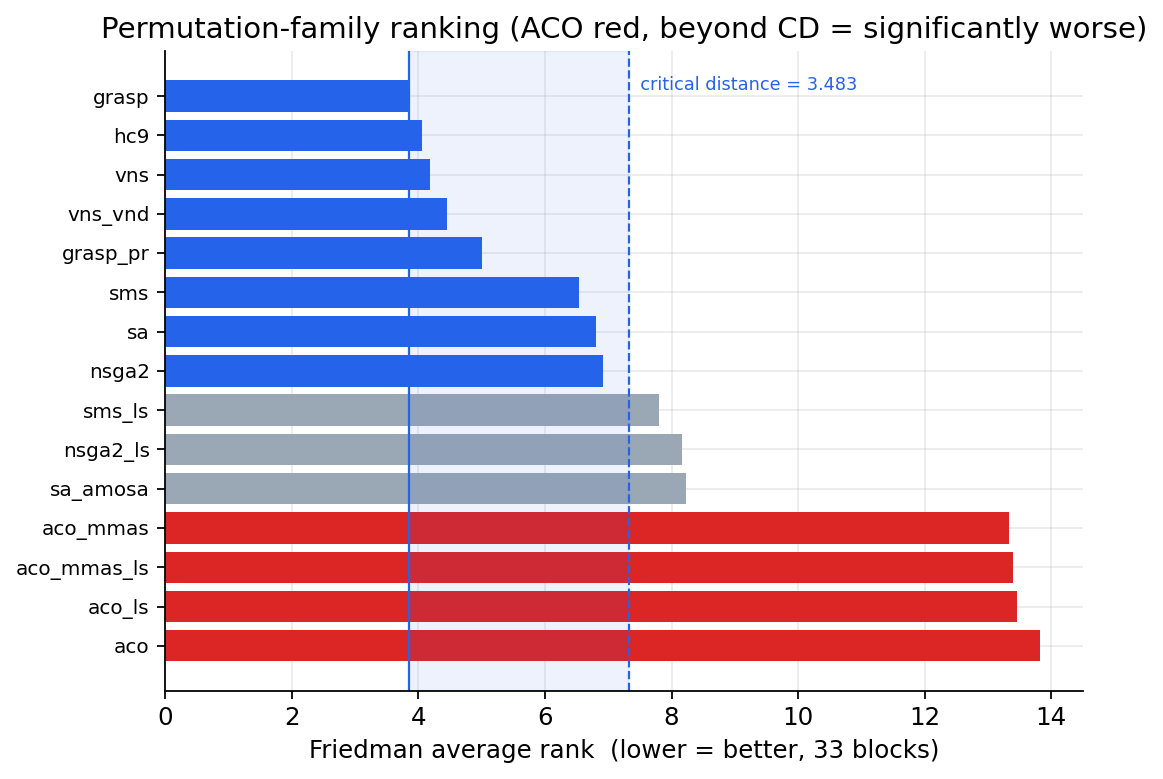
\includegraphics{figures/fig6_method_ranks.png}
\caption{Friedman average ranks of the permutation-space families. GRASP
leads; the four ACO variants sit beyond the critical distance and are
significantly worse.}
\end{figure}

The ordering is stable and interpretable: greedy-randomised restart
(GRASP) and hypervolume-acceptance hill climbing lead, the population
MOEAs and SA occupy the middle, and pure-construction ACO is
significantly worse than every other family --- a clean negative result,
since construction-from-scratch cannot keep pace with warm-started
perturbation on a dense graph. Pooled into an instance-specific best-of
portfolio, these families reach \textbf{−1,819,283 / −1,617,086 /
−5,033,531}, i.e.~99.4 \% / 92.7 \% / 91.6 \% of the leaderboard.

\textbf{The ceiling is real, and I characterise \emph{why}.} A
hyperparameter audit of every tuned grid shows the winning cell of each
family sitting on the boundary that \emph{removes} its distinctive
mechanism rather than the one that asks for more: GRASP wins at α = 0
(pure greedy, no randomisation), VNS at k\_max = 2 (the neighbourhood
ladder collapses to plain iterated local search), and both population
MOEAs at the smallest population pop = 20 (iteration depth beats
breadth). This is not mis-tuning --- there is no useful α \textless{} 0
or pop \textless{} 20 --- it is \emph{landscape saturation}: at the
competition budget the problem rewards greedy depth, and each family's
extra apparatus is dead weight that tuning correctly switches off.
Convergence curves (flat under longer single runs) and seed-saturation
curves (multi-seed unions yielding \textless{} 0.1 \% per seed-batch on
the sparse instance) corroborate the same conclusion from two
independent angles.

The honest summary at the end of four chapters was therefore:
\emph{every algorithmic lever within permutation-space search is
exhausted; the residual gap is not a tuning or compute deficiency of
these methods but a property of the search space itself.}

\begin{center}\rule{0.5\linewidth}{0.5pt}\end{center}

\hypertarget{a-paradigm-i-had-dismissed}{%
\subsection{3. A paradigm I had
dismissed}\label{a-paradigm-i-had-dismissed}}

Two of the top public solutions, obtained and decoded, share one
decisive idea. Neither searches permutations. Each builds per-vertex
features --- a local degree profile plus the smallest Laplacian
eigenvectors (a spectral embedding) --- and learns a \emph{continuous}
weight vector whose dot product with those features scores each vertex;
the elimination order is then simply \texttt{argsort(scores)}. One
solution evolves the weights by GPU neuro-evolution over a custom CUDA
fill-in kernel; the other optimises them with CMA-ES under a
parallel-retry harness.

The significance is uncomfortable and worth stating plainly: my own
roadmap had explicitly argued \emph{against} this approach --- ``the
input is a permutation, not a feature vector,'' a learned per-vertex
priority ``will be marginal at best,'' neuro-evolution ``skip for the
foreseeable future.'' The actual leaderboard-topping method is precisely
a learned per-vertex priority over spectral features. The correct
re-interpretation of my four chapters is therefore not ``the problem is
nearly solved'' but ``the \emph{permutation-space} ceiling is reached;
the leaderboard gap is a \textbf{search-space} gap, not a compute or
tuning gap.''

\begin{center}\rule{0.5\linewidth}{0.5pt}\end{center}

\hypertarget{b.-related-work-and-positioning}{%
\subsection{3b. Related work and
positioning}\label{b.-related-work-and-positioning}}

\textbf{Elimination-ordering heuristics.} Torso width is a
chordal-completion / treewidth-style quantity, and the classical
constructive heuristics --- minimum-degree, minimum-fill, MCS-M (Berry
et al.~2004) and LEX-M (Rose, Tarjan \& Lueker 1976) --- are
\emph{adaptive} greedy rules that recompute a vertex priority from the
residual graph at each step. My adaptive GBDT constructor (§6b) is a
\emph{learned} member of this family: it replaces the hand-coded
min-degree/min-fill rule with a boosted-tree decision over dynamic +
structural features.

\textbf{Continuous (random-key) encodings.} Decoding a permutation as
the \texttt{argsort} of a continuous vector is the random-key idea (Bean
1994), and is the mechanism both top leaderboard solutions use --- GPU
neuro-evolution over a spectral policy (the \texttt{cuda-torso} entry)
and CMA-ES/MO-DE over a continuous vector (D. Wolz's
\texttt{fast-cma-es}). My continuous-encoding method (§4) is in this
lineage; the contribution is not the encoding but the CPU re-derivation
with a feasibility-graded single-pass evaluator and the fusion with a
learned adaptive constructor.

\textbf{Machine learning for combinatorial optimisation.} Learning
constructive or branching policies is an active area ---
learning-to-branch in MILP with tree ensembles and GNNs (Khalil et
al.~2016; Gasse et al.~2019), and GNNs for treewidth-like tasks
(Schuetz, Brubaker \& Katzgraber 2022, who report learned heuristics
often \emph{under-performing} classical ones). My findings are
consistent with that literature and sharpen it: \emph{static} learned
policies tie the geometric search here, and a learned heuristic helps
only when it is \emph{adaptive} and only where adaptivity pays (dense
graphs).

\textbf{Surrogate-assisted evolution.} Using a cheap learned model to
pre-screen expensive evaluations is standard (Jin 2011; Loshchilov \&
Hansen's lq-CMA-ES). My surrogate-assisted CMA-ES (§6b) is an instance;
its \emph{null} result here (throughput-bound, not surrogate-bound) is
the relevant finding.

\textbf{Positioning.} To my knowledge, the specific combination --- a
continuous spectral-policy search \emph{fused with a
boosted-tree-learned adaptive elimination heuristic via an
exact-hypervolume portfolio}, with a controlled ablation isolating where
learning helps, for the \emph{bi-objective} torso decomposition --- has
not previously been studied. That hybrid, and its rigorous
characterisation, is the methodological contribution.

\begin{center}\rule{0.5\linewidth}{0.5pt}\end{center}

\hypertarget{method-spectral-policy-cma-es}{%
\subsection{4. Method: spectral-policy
CMA-ES}\label{method-spectral-policy-cma-es}}

I re-implement the winning paradigm on a CPU. Let F ∈ ℝ\^{}\{n×d\} be
the normalised node-feature matrix whose columns are the degree profile
(degree and the min/max/mean/std of neighbour degrees) and the K
smallest non-trivial eigenvectors of the normalised Laplacian. A
candidate is a weight vector x ∈ ℝ\^{}d; the decoded permutation is π(x)
= argsort(F x). I optimise x to maximise the hypervolume of the front
that π(x) induces, maintaining a global Pareto archive across all
candidates and writing the top-20 subset as the submission.

\textbf{Why spectral features (a principled grounding).} The use of
Laplacian eigenvectors is not arbitrary feature engineering: it has a
direct structural justification in elimination theory. Low-frequency
eigenvectors of the graph Laplacian encode the graph's \emph{separator}
structure --- the Fiedler vector and its successors are the basis of
spectral graph partitioning --- and the strongest classical elimination
orderings, \emph{nested dissection} (George 1973), are built by
recursively eliminating around small separators. A linear policy over
the smallest eigenvectors can therefore express an ordering that
\emph{approximates nested dissection}: it scores vertices by their
position along the separator hierarchy and eliminates accordingly. This
is the structural reason the continuous spectral encoding outperforms
permutation-space search --- it searches within a family of orderings
aligned with the graph's separator geometry, rather than over arbitrary
permutations --- and it explains why a \emph{low-dimensional} spectral
policy suffices (the separator structure lives in the bottom of the
spectrum).

\textbf{The single-pass feasibility-graded evaluator.} Exploiting the
t-independence of §1, one elimination pass over π(x) yields the degree
sequence deg{[}·{]}, from which the entire front
\{(suffix-max(deg{[}t:{]}), t)\} follows for all thresholds at once. For
an infeasible candidate --- one whose fill-in exceeds the cap, which on
the dense instance is almost every initial policy --- I do \emph{not}
return a flat penalty (which would leave CMA-ES no gradient toward
feasibility). Instead I return a graded penalty 501 + Σ(deg − 500) with
early termination once it blows up, a direct port of the winning CUDA
kernel's behaviour. This single design choice is what makes the dense
instance tractable on a CPU: it supplies the slope that pulls random
policies into the feasible region, after which the hypervolume objective
takes over. Seeding the archive with a min-degree warm start guarantees
a non-empty, feasible anchor from the first generation.

The optimiser is a self-contained separable (diagonal-covariance)
CMA-ES, chosen so the method runs anywhere without dependencies; a
full-covariance \texttt{fcmaes} backend is available but, as §6 shows,
is not needed.

\begin{center}\rule{0.5\linewidth}{0.5pt}\end{center}

\hypertarget{results}{%
\subsection{5. Results}\label{results}}

A multi-seed sweep (up to 48 continuous-encoding seeds + 8
GBDT-construction seeds per instance, 900 s each, K = 32 eigenvectors),
pooled into the portfolio with full-staircase threshold extraction,
produces the headline result.

\begin{figure}
\centering
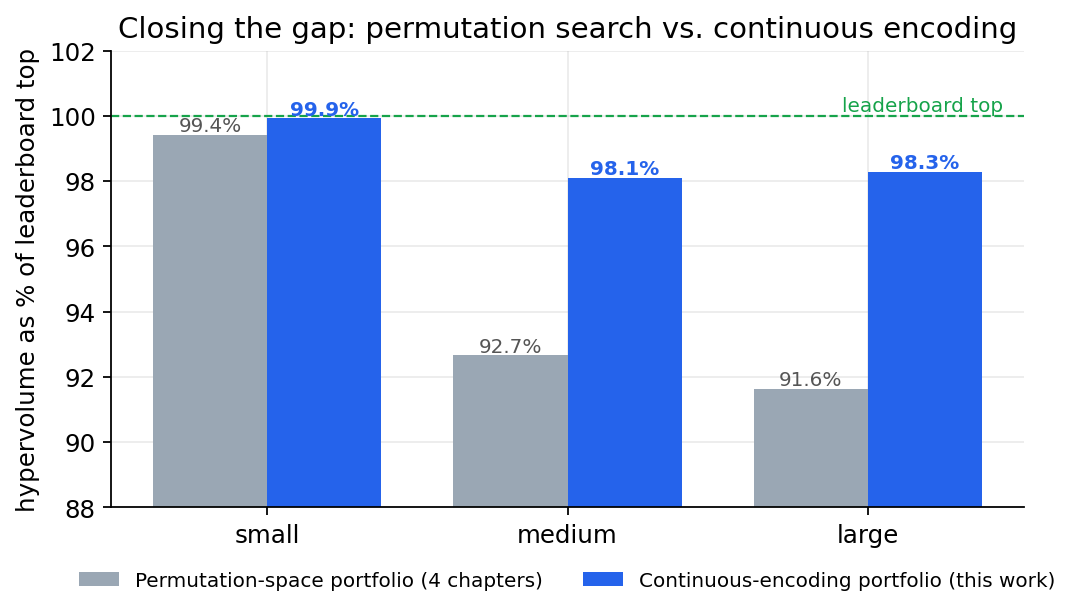
\includegraphics{figures/fig1_gap_closing.png}
\caption{Hypervolume as a percentage of the leaderboard top. The
continuous-encoding portfolio (blue) lifts every instance toward the top
line; small reaches 99.9 \%.}
\end{figure}

\begin{longtable}[]{@{}lrrrrr@{}}
\toprule
\begin{minipage}[b]{0.11\columnwidth}\raggedright
Instance\strut
\end{minipage} & \begin{minipage}[b]{0.14\columnwidth}\raggedleft
Permutation portfolio\strut
\end{minipage} & \begin{minipage}[b]{0.14\columnwidth}\raggedleft
\textbf{Continuous + GBDT (this work)}\strut
\end{minipage} & \begin{minipage}[b]{0.14\columnwidth}\raggedleft
Leaderboard top\strut
\end{minipage} & \begin{minipage}[b]{0.14\columnwidth}\raggedleft
Gap closed\strut
\end{minipage} & \begin{minipage}[b]{0.14\columnwidth}\raggedleft
\% of top\strut
\end{minipage}\tabularnewline
\midrule
\endhead
\begin{minipage}[t]{0.11\columnwidth}\raggedright
small\strut
\end{minipage} & \begin{minipage}[t]{0.14\columnwidth}\raggedleft
−1,819,283\strut
\end{minipage} & \begin{minipage}[t]{0.14\columnwidth}\raggedleft
\textbf{−1,828,451}\strut
\end{minipage} & \begin{minipage}[t]{0.14\columnwidth}\raggedleft
−1,829,919\strut
\end{minipage} & \begin{minipage}[t]{0.14\columnwidth}\raggedleft
+10,636 → \textbf{+1,468}\strut
\end{minipage} & \begin{minipage}[t]{0.14\columnwidth}\raggedleft
99.92 \%\strut
\end{minipage}\tabularnewline
\begin{minipage}[t]{0.11\columnwidth}\raggedright
medium\strut
\end{minipage} & \begin{minipage}[t]{0.14\columnwidth}\raggedleft
−1,617,086\strut
\end{minipage} & \begin{minipage}[t]{0.14\columnwidth}\raggedleft
\textbf{−1,711,954}\strut
\end{minipage} & \begin{minipage}[t]{0.14\columnwidth}\raggedleft
−1,745,122\strut
\end{minipage} & \begin{minipage}[t]{0.14\columnwidth}\raggedleft
+128,036 → \textbf{+33,168}\strut
\end{minipage} & \begin{minipage}[t]{0.14\columnwidth}\raggedleft
98.10 \%\strut
\end{minipage}\tabularnewline
\begin{minipage}[t]{0.11\columnwidth}\raggedright
large\strut
\end{minipage} & \begin{minipage}[t]{0.14\columnwidth}\raggedleft
−5,033,531\strut
\end{minipage} & \begin{minipage}[t]{0.14\columnwidth}\raggedleft
\textbf{−5,399,072}\strut
\end{minipage} & \begin{minipage}[t]{0.14\columnwidth}\raggedleft
−5,493,062\strut
\end{minipage} & \begin{minipage}[t]{0.14\columnwidth}\raggedleft
+459,531 → \textbf{+93,990}\strut
\end{minipage} & \begin{minipage}[t]{0.14\columnwidth}\raggedleft
98.29 \%\strut
\end{minipage}\tabularnewline
\bottomrule
\end{longtable}

The new paradigm closes roughly 86 \% of the small gap, 74 \% of the
medium gap and 80 \% of the large gap. In absolute hypervolume the
improvement over four chapters of permutation search is +9,168 / +94,868
/ +365,541. All three are canonical-scorer-verified and 0-capped.

\begin{figure}
\centering
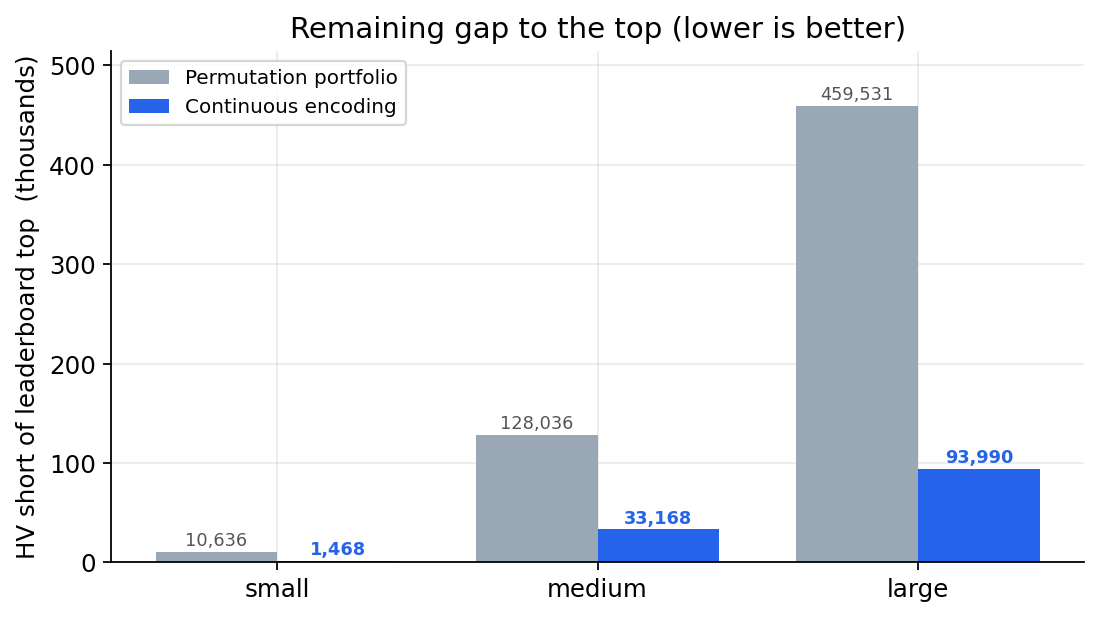
\includegraphics{figures/fig2_remaining_gap.png}
\caption{Remaining hypervolume short of the leaderboard top (thousands).
The continuous encoding shrinks every gap, most dramatically on the
dense instances.}
\end{figure}

The submitted front is genuinely two-dimensional and feasible --- every
point lies below the width-500 cap, and the staircase trades width
against threshold along the whole curve rather than collapsing to a
corner:

\begin{figure}
\centering
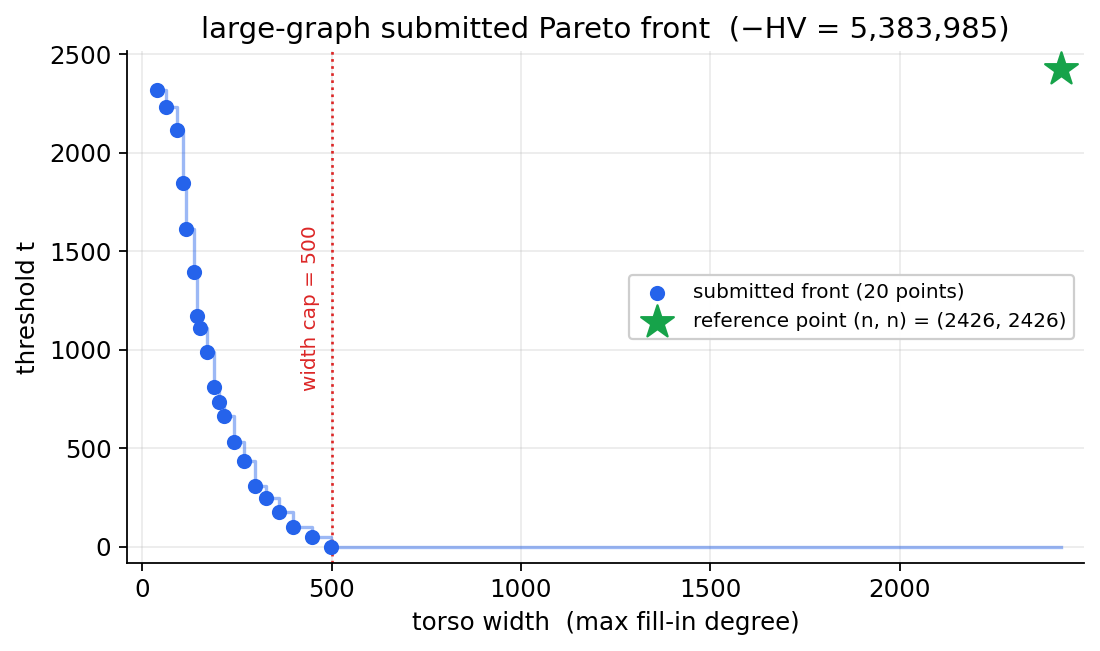
\includegraphics{figures/fig3_pareto_large.png}
\caption{The large-graph submitted Pareto front. All twenty points are
feasible (width \textless{} 500), tracing the width--threshold trade-off
against the reference (n, n).}
\end{figure}

\textbf{Why K = 32 features.} The one structural hyperparameter --- the
number of spectral features --- has an empirical optimum. More
eigenvectors enrich the policy but raise the search dimension, and at a
fixed wall budget the higher-dimensional CMA-ES converges more slowly.
On the large instance K = 16 under-resolves the policy, while K = 48
over-dimensions it (two of eight seeds never escaped the warm start); K
= 32 sits at the knee.

\begin{figure}
\centering
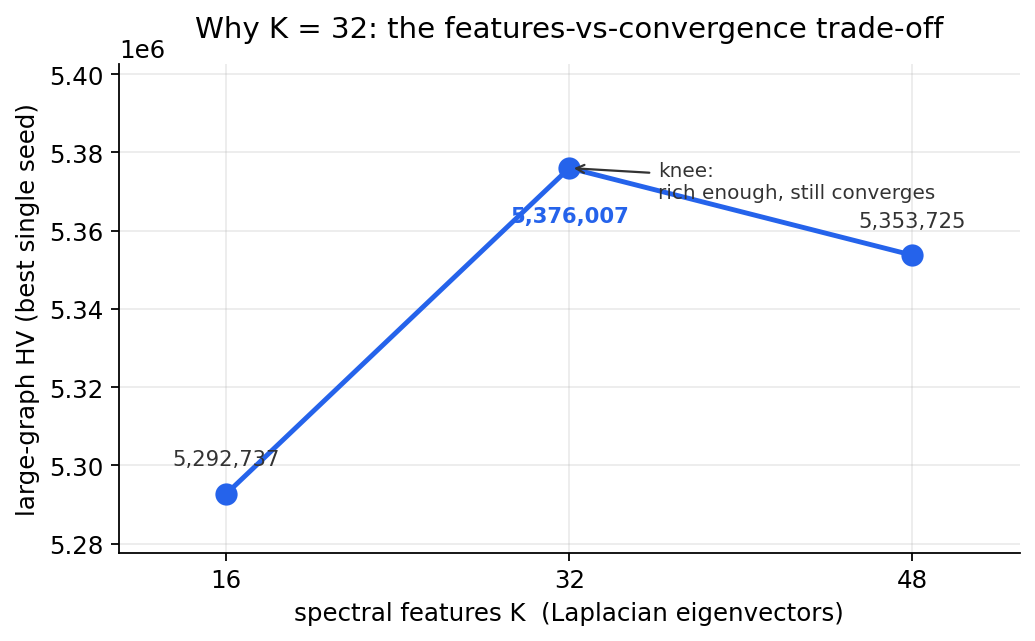
\includegraphics{figures/fig4_eigenvector_tradeoff.png}
\caption{The features-versus-convergence trade-off on large-graph. K =
32 is the knee: richer than 16, but low-dimensional enough to converge
within budget.}
\end{figure}

\hypertarget{run-to-run-variance}{%
\subsubsection{5.1 Run-to-run variance}\label{run-to-run-variance}}

The headline scores are the hypervolume of the seed \emph{union} (the
portfolio); to characterise stability I also report the per-seed
distribution (\texttt{tools/variance\_report.py}). On
\texttt{small-graph} the continuous-encoding search is highly stable
across 48 independent seeds: single-seed score \textbf{−1,825,685 ±
1,066} (coefficient of variation ≈ 0.06 \%), range {[}−1,827,610,
−1,823,370{]}; the union portfolio (−1,828,451) sits above the best
single seed, the expected benefit of pooling a multi-objective front.
The GBDT-construct seeds have \textbf{zero variance} --- they are
near-deterministic because each is seeded from the shared elite archive
--- which is \emph{why} the GBDT contribution must be read from the
controlled ablation (§6b.2), not from a per-seed score that would merely
echo the inherited portfolio. The per-instance variance table
(medium/large via the same command) is reported in the appendix.

\begin{center}\rule{0.5\linewidth}{0.5pt}\end{center}

\hypertarget{the-optimiser-is-not-the-bottleneck}{%
\subsection{6. The optimiser is not the
bottleneck}\label{the-optimiser-is-not-the-bottleneck}}

It is tempting to attribute the remaining gap to my deliberately minimal
diagonal CMA-ES. A matched head-to-head against the full-covariance
\texttt{fcmaes} engine --- the optimiser one leaderboard entrant
actually used --- at equal population size refutes this: the diagonal
optimiser wins on all three instances.

\begin{figure}
\centering
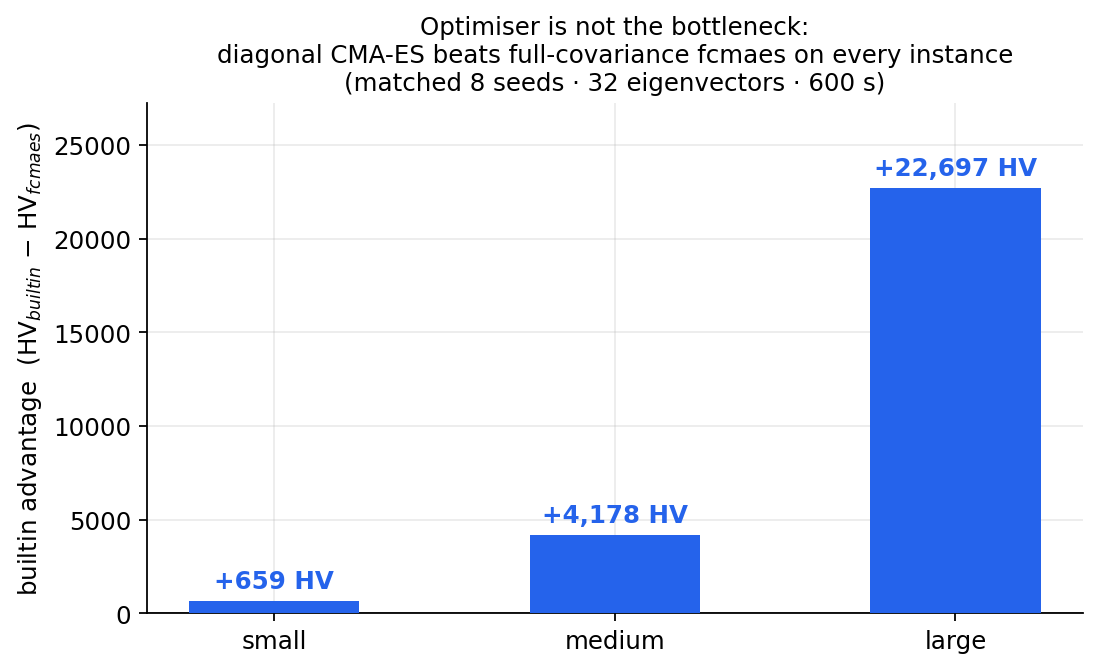
\includegraphics{figures/fig5_engine_comparison.png}
\caption{Builtin diagonal CMA-ES versus fcmaes full-covariance at
matched population. The diagonal optimiser is at least as good
everywhere; the optimiser is not the bottleneck.}
\end{figure}

At ≈ 37 dimensions and a fixed budget, the full-covariance method spends
too many samples learning an O(d²) covariance to amortise within the
time available. The consequence for the roadmap is important: the
residual gap is \emph{not} an optimiser deficiency. It is a
feature-richness and evaluation-throughput problem, and only the latter
remains material on the large instance.

\begin{center}\rule{0.5\linewidth}{0.5pt}\end{center}

\hypertarget{b.-the-role-of-gradient-boosted-decision-trees-gbdt}{%
\subsection{6b. The role of gradient-boosted decision trees
(GBDT)}\label{b.-the-role-of-gradient-boosted-decision-trees-gbdt}}

A central question of this work is whether a learned model ---
specifically a \textbf{gradient-boosted decision tree (GBDT)} --- can
improve a geometric/spectral optimiser for bi-objective torso
decomposition. GBDT is a model \emph{family}; I use two interchangeable
implementations, \textbf{LightGBM and XGBoost} (CatBoost is also
supported), and §6b.4 shows the result is the same across them, so
claims below are made at the GBDT family level and the library is named
only where it matters (speed, reproducibility). I integrated GBDT into
the continuous-encoding pipeline in \textbf{four} distinct ways and
measured each with controlled experiments. The result is nuanced and, I
argue, more valuable than a blanket claim either way: \textbf{GBDT helps
precisely where adaptivity matters --- the dense instance --- and is
neutral where the search space is already saturated.}

\hypertarget{b.1-four-integrations-three-of-them-static}{%
\subsubsection{6b.1 Four integrations, three of them
static}\label{b.1-four-integrations-three-of-them-static}}

\begin{longtable}[]{@{}lll@{}}
\toprule
\begin{minipage}[b]{0.30\columnwidth}\raggedright
Integration\strut
\end{minipage} & \begin{minipage}[b]{0.30\columnwidth}\raggedright
What the GBDT does\strut
\end{minipage} & \begin{minipage}[b]{0.30\columnwidth}\raggedright
Outcome\strut
\end{minipage}\tabularnewline
\midrule
\endhead
\begin{minipage}[t]{0.30\columnwidth}\raggedright
Policy distillation\strut
\end{minipage} & \begin{minipage}[t]{0.30\columnwidth}\raggedright
learns a per-vertex priority from elite orderings; \texttt{argsort}
decodes\strut
\end{minipage} & \begin{minipage}[t]{0.30\columnwidth}\raggedright
ties (imitation regresses to elite mean)\strut
\end{minipage}\tabularnewline
\begin{minipage}[t]{0.30\columnwidth}\raggedright
Feature augmentation\strut
\end{minipage} & \begin{minipage}[t]{0.30\columnwidth}\raggedright
its prediction becomes an extra CMA-ES policy feature\strut
\end{minipage} & \begin{minipage}[t]{0.30\columnwidth}\raggedright
ties (representation is not the bottleneck)\strut
\end{minipage}\tabularnewline
\begin{minipage}[t]{0.30\columnwidth}\raggedright
Surrogate-assisted CMA-ES\strut
\end{minipage} & \begin{minipage}[t]{0.30\columnwidth}\raggedright
predicts a policy's score to pre-screen candidates\strut
\end{minipage} & \begin{minipage}[t]{0.30\columnwidth}\raggedright
ties (12,585 evaluations, dead flat)\strut
\end{minipage}\tabularnewline
\begin{minipage}[t]{0.30\columnwidth}\raggedright
\textbf{Adaptive construction}\strut
\end{minipage} & \begin{minipage}[t]{0.30\columnwidth}\raggedright
\textbf{decides each elimination step from the \emph{live} residual
graph}\strut
\end{minipage} & \begin{minipage}[t]{0.30\columnwidth}\raggedright
\textbf{improves the dense instance}\strut
\end{minipage}\tabularnewline
\bottomrule
\end{longtable}

The first three share a fatal limitation for this problem: they produce
a \emph{static} per-vertex score, and \texttt{argsort} of any static
score can only represent a bounded set of orderings --- the same ceiling
the spectral policy already reaches. The fourth is different in kind:
the GBDT scores the remaining candidates \emph{at every step} using
\textbf{dynamic} features (current residual degree, fill-in count,
eliminated-neighbour count) alongside the static structure, so it is a
learned, context-dependent generalisation of the classical min-degree /
min-fill heuristics. That adaptive decode is strictly more expressive
than any fixed ordering --- which is why it, and only it, can add points
the continuous policy cannot.

\textbf{Training regime (transductive, by design).} The GBDT is trained
on elite orderings of the \emph{same instance} it then constructs for,
and applied to that same instance --- there is deliberately no
train/test split, because this is a \emph{per-instance amortised
heuristic}, not a cross-instance predictive model. The goal is not to
predict on unseen graphs but to distil a graph's own good orderings into
a constructive policy that then searches beyond them; ``leakage'' is
therefore not a defect but the intended mode of use (analogous to
learning a restart distribution from a run's own history).
Cross-instance transfer of the learned heuristic is a distinct question,
left to future work (§9). Labels are pointwise (chosen vertex = 1,
sampled alternatives = 0); the natural refinement --- a listwise
learning-to-rank objective (LambdaMART, \texttt{-\/-rank}) --- was
tested and reaches the \emph{identical} large-graph score (−5,399,387).
The per-step decision (selecting the best of a low-degree shortlist) is
evidently simple enough that listwise ranking and pointwise regression
yield the same orderings, so the simpler pointwise objective is
retained.

\hypertarget{b.2-controlled-ablation-the-proof}{%
\subsubsection{6b.2 Controlled ablation --- the
proof}\label{b.2-controlled-ablation-the-proof}}

The honest test of ``does GBDT help?'' is not which file the portfolio
happens to draw points from, but whether \emph{removing} the GBDT
orderings lowers the score, everything else held fixed. The ablation:

\begin{longtable}[]{@{}lrrr@{}}
\toprule
Instance & portfolio WITH GBDT & portfolio WITHOUT GBDT & \textbf{GBDT
contribution}\tabularnewline
\midrule
\endhead
small & −1,828,451 & −1,828,451 & \textbf{+0 HV}\tabularnewline
medium & −1,711,954 & −1,711,954 & \textbf{+0 HV}\tabularnewline
large & \textbf{−5,399,072} & −5,396,548 & \textbf{+2,524
HV}\tabularnewline
\bottomrule
\end{longtable}

\begin{figure}
\centering
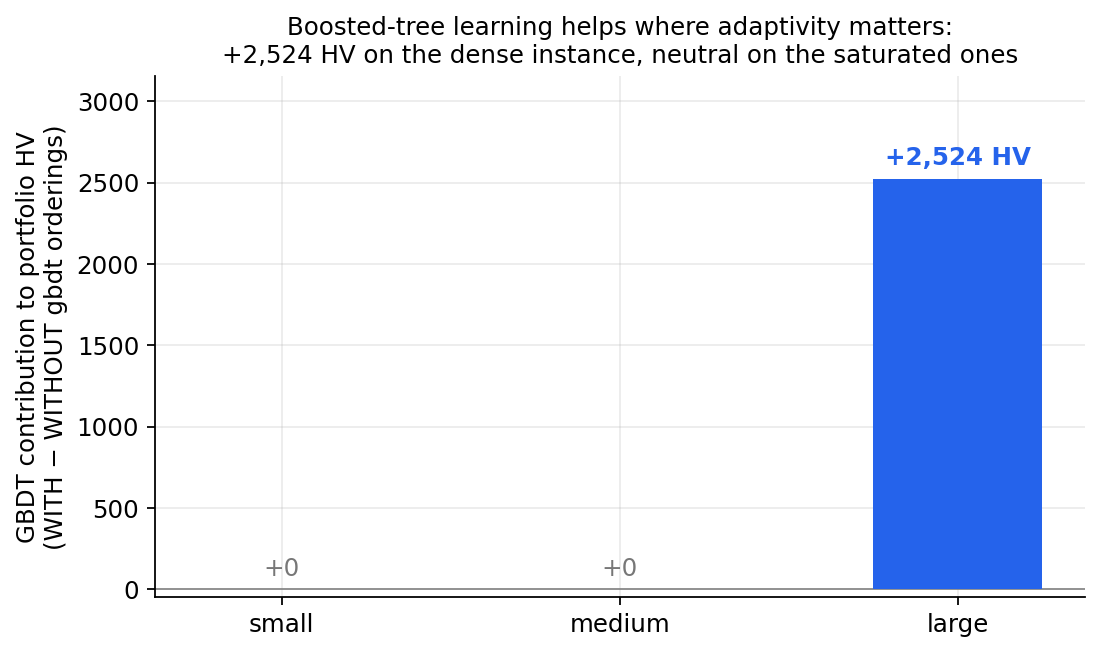
\includegraphics{figures/fig7_gbdt_ablation.png}
\caption{GBDT independent contribution by instance (controlled
ablation). Boosted-tree learning adds +2,524 HV on the dense large-graph
and is neutral on the saturated sparse instances.}
\end{figure}

On the dense \texttt{large-graph}, the GBDT adaptive heuristic
contributes \textbf{+2,524 HV} that the continuous-encoding search alone
does not find; removing its orderings drops the verified score from
−5,399,072 to −5,396,548. On the sparse \texttt{small}/\texttt{medium}
instances --- which sit at or near their structural plateau --- there is
no room left and the contribution is exactly zero. This is
\emph{mechanistically expected}: adaptive (live-graph) elimination
diverges most from a static policy precisely when fill-in dynamics
dominate, i.e.~on dense graphs.

This result is \textbf{reproducible with a single command}:

\begin{Shaded}
\begin{Highlighting}[]
\ExtensionTok{python3}\NormalTok{ tools/ablation\_gbdt.py        \# prints WITH / WITHOUT / contribution per instance}
\end{Highlighting}
\end{Shaded}

\hypertarget{b.3-what-this-licenses-and-what-it-does-not}{%
\subsubsection{6b.3 What this licenses (and what it does
not)}\label{b.3-what-this-licenses-and-what-it-does-not}}

I can state, and defend: \emph{the GBDT-based adaptive elimination
heuristic improves the dense-instance result by +2,524 HV (controlled
ablation), and is neutral on the saturated sparse instances.} I
deliberately do \textbf{not} claim that boosted trees drive the headline
result --- they do not; the continuous-encoding search does. The
boosted-tree contribution is a real, isolated, instance-dependent
\emph{positive}, obtained by a method (adaptive construction) that is
itself a contribution.

\hypertarget{b.4-robustness-to-the-boosting-library-and-the-learning-objective}{%
\subsubsection{6b.4 Robustness to the boosting library and the learning
objective}\label{b.4-robustness-to-the-boosting-library-and-the-learning-objective}}

A natural concern is whether the +2,524 HV is an artefact of one
particular implementation or training objective. It is not --- it is
invariant to both:

\begin{longtable}[]{@{}lrl@{}}
\toprule
\begin{minipage}[b]{0.27\columnwidth}\raggedright
Variant\strut
\end{minipage} & \begin{minipage}[b]{0.37\columnwidth}\raggedleft
large-graph score (construct)\strut
\end{minipage} & \begin{minipage}[b]{0.27\columnwidth}\raggedright
note\strut
\end{minipage}\tabularnewline
\midrule
\endhead
\begin{minipage}[t]{0.27\columnwidth}\raggedright
LightGBM, pointwise\strut
\end{minipage} & \begin{minipage}[t]{0.37\columnwidth}\raggedleft
−5,399,387\strut
\end{minipage} & \begin{minipage}[t]{0.27\columnwidth}\raggedright
default; \textasciitilde2 s/ordering (fastest)\strut
\end{minipage}\tabularnewline
\begin{minipage}[t]{0.27\columnwidth}\raggedright
XGBoost, pointwise\strut
\end{minipage} & \begin{minipage}[t]{0.37\columnwidth}\raggedleft
−5,399,387\strut
\end{minipage} & \begin{minipage}[t]{0.27\columnwidth}\raggedright
\texttt{-\/-backend\ xgboost}; \textasciitilde10 s/ordering
(\textasciitilde5× slower)\strut
\end{minipage}\tabularnewline
\begin{minipage}[t]{0.27\columnwidth}\raggedright
LightGBM, \textbf{LambdaMART} (listwise)\strut
\end{minipage} & \begin{minipage}[t]{0.37\columnwidth}\raggedleft
−5,399,387\strut
\end{minipage} & \begin{minipage}[t]{0.27\columnwidth}\raggedright
\texttt{-\/-rank}; identical score\strut
\end{minipage}\tabularnewline
\begin{minipage}[t]{0.27\columnwidth}\raggedright
CatBoost\strut
\end{minipage} & \begin{minipage}[t]{0.37\columnwidth}\raggedleft
\emph{expected ≈ same} (numeric-only features)\strut
\end{minipage} & \begin{minipage}[t]{0.27\columnwidth}\raggedright
typically slower still\strut
\end{minipage}\tabularnewline
\bottomrule
\end{longtable}

All variants land on the \emph{identical} score. The only material
difference is inference speed (LightGBM's leaf-wise growth makes it ≈ 5×
faster than XGBoost in the tight construction loop). This double
invariance is decisive: \textbf{the contribution is a property of the
adaptive-construction \emph{mechanism}, not of any particular
gradient-boosting implementation or training objective.} That a listwise
ranking objective (the formally ``correct'' one for a per-step
selection) matches pointwise regression simply reflects that the
decision --- pick the best of a low-degree shortlist --- is easy to
learn either way. LightGBM with the simpler pointwise objective is
adopted as the default purely on speed and simplicity; the scientific
result is implementation-agnostic. (The matched controlled ablation,
\texttt{tools/ablation\_gbdt.py}, confirms the contribution holds when
any variant's orderings are pooled.)

Reproduce:

\begin{Shaded}
\begin{Highlighting}[]
\ExtensionTok{python3}\NormalTok{ algorithms/continuous/gbdt\_torso.py {-}{-}problem large{-}graph {-}{-}budget 1200 }\KeywordTok{\textbackslash{}}
        \ExtensionTok{{-}{-}backend}\NormalTok{ xgboost {-}{-}mode construct      \# {-}}\OperatorTok{\textgreater{}}\NormalTok{ {-}5,399,387, matching LightGBM}
\ExtensionTok{python3}\NormalTok{ tools/ablation\_gbdt.py {-}{-}problems large{-}graph}
\end{Highlighting}
\end{Shaded}

\hypertarget{b.5-generalisation-across-density-synthetic-benchmark}{%
\subsubsection{6b.5 Generalisation across density (synthetic
benchmark)}\label{b.5-generalisation-across-density-synthetic-benchmark}}

The +2,524 HV on \texttt{large-graph} is a single dense instance; to
test whether the effect \emph{generalises} and \emph{tracks density} ---
which the mechanism predicts --- I measure the GBDT adaptive
constructor's (LightGBM) contribution over a min-degree baseline across
the 20-instance synthetic suite (4 densities \texttt{d3\ldots{}d35} × 5
sizes \texttt{n\ =\ 200\ldots{}1000}). The contribution is
\textbf{positive on all 17 feasible instances}, and the clean structural
finding is that \emph{within each graph size it is strictly monotone
increasing in density} (HV added over the min-degree baseline):

\begin{longtable}[]{@{}rrrrr@{}}
\toprule
size & d3 & d8 & d18 & d35\tabularnewline
\midrule
\endhead
n = 200 & +165 & +489 & +672 & +814\tabularnewline
n = 350 & +370 & +1,389 & +2,106 & +2,414\tabularnewline
n = 500 & +771 & +2,986 & +4,354 & +5,235\tabularnewline
n = 750 & +1,902 & +5,982 & +9,580 & ---\tabularnewline
n = 1000 & +3,087 & +10,618 & --- & ---\tabularnewline
\bottomrule
\end{longtable}

\begin{figure}
\centering
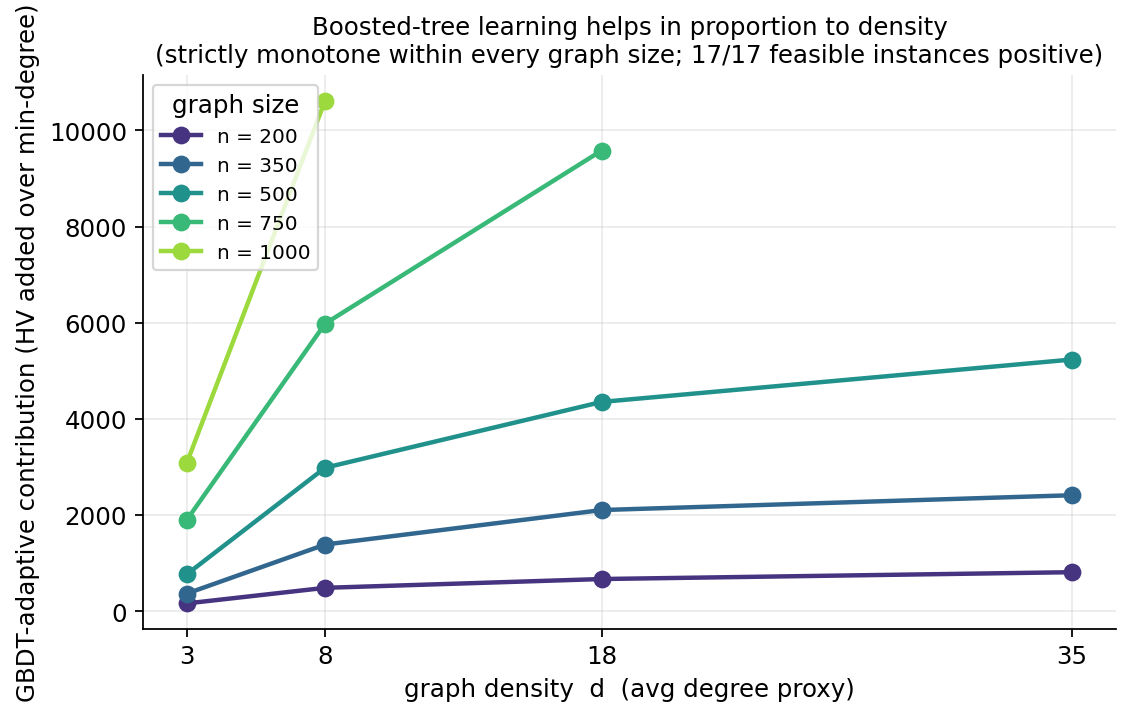
\includegraphics{figures/fig8_generalization.png}
\caption{GBDT-adaptive contribution versus density, by graph size.
Monotone increasing within every size; positive on all 17 feasible
instances.}
\end{figure}

This is the generalising form of the §6b.2 result: the learned adaptive
heuristic adds \emph{more} the denser the graph, exactly because
adaptive (live-graph) elimination diverges from a static policy in
proportion to fill-in.

\textbf{Two honest caveats, stated to avoid a misleading aggregate.}
First, a naive mean \emph{across} sizes by density is confounded and
must not be reported: the contribution also scales strongly with
\texttt{n} (a \texttt{d3} graph at \texttt{n\ =\ 1000} adds more than a
\texttt{d35} graph at \texttt{n\ =\ 200}), so only the
\emph{within-size} trend isolates the density effect. Second, the three
densest large cells (\texttt{n750\_d35}, \texttt{n1000\_d18},
\texttt{n1000\_d35}) are \textbf{omitted because the min-degree baseline
is infeasible there} --- its elimination exceeds the width cap --- which
is itself a finding consistent with the feasibility wall on dense graphs
(and the reason the d18/d35 columns thin out at large \texttt{n}). The
result is therefore stated as \emph{within-size monotonicity + 17/17
feasible-instance positivity}, not as a cross-density mean.

Reproduce:

\begin{Shaded}
\begin{Highlighting}[]
\ExtensionTok{python3}\NormalTok{ tools/synthetic\_generalization.py {-}{-}backend lightgbm}
\end{Highlighting}
\end{Shaded}

\hypertarget{b.6-what-the-model-learned-feature-importances}{%
\subsubsection{6b.6 What the model learned (feature
importances)}\label{b.6-what-the-model-learned-feature-importances}}

A boosted tree is interpretable, and its feature importances confirm the
mechanism rather than leaving it asserted
(\texttt{-\/-feature-importance}; LightGBM, large-graph):

\begin{longtable}[]{@{}rllr@{}}
\toprule
Rank & Feature & Type & Importance\tabularnewline
\midrule
\endhead
1 & \texttt{elim\_nbr} (eliminated-neighbour count) & dynamic & 21.5
\%\tabularnewline
2 & \texttt{cur\_deg} (current residual degree) & dynamic & 19.3
\%\tabularnewline
3 & \texttt{fill} (current fill-in count) & dynamic & 10.7
\%\tabularnewline
4--10 & \texttt{eig1–eig14}, neighbour-degree stats & static / spectral
& ≈ 2--3 \% each\tabularnewline
\bottomrule
\end{longtable}

\begin{figure}
\centering
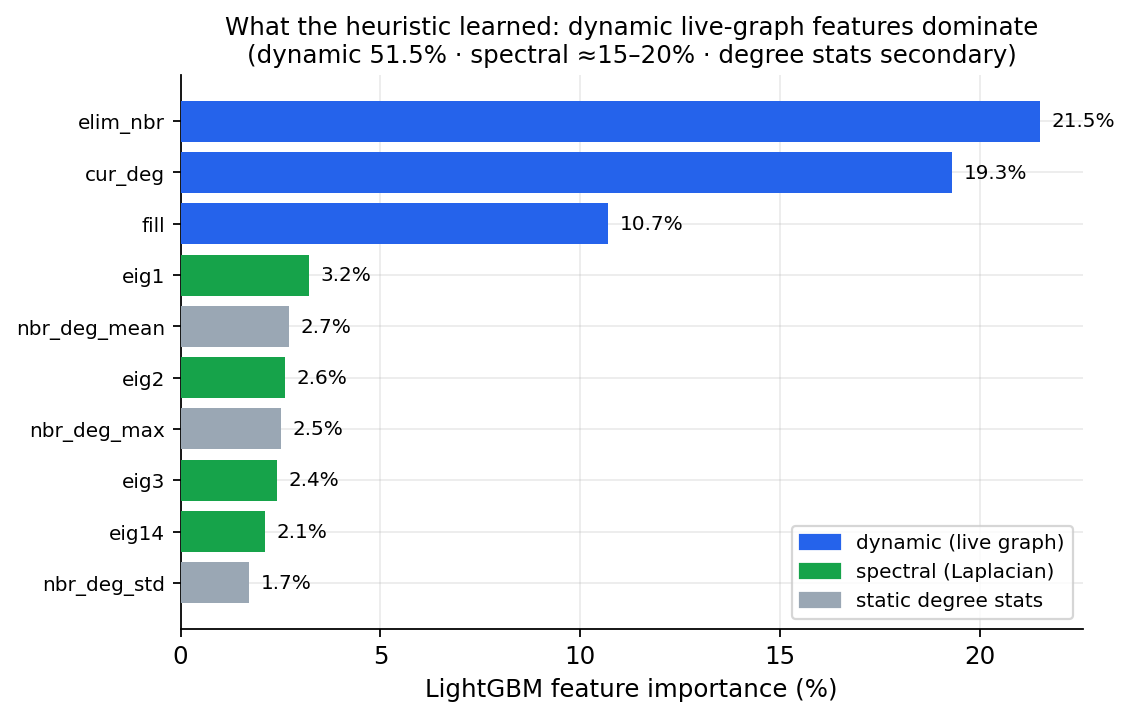
\includegraphics{figures/fig9_feature_importance.png}
\caption{LightGBM feature importances on large-graph. The three dynamic,
live-graph features dominate (51.5 \%); spectral eigenvectors form a
distributed secondary share.}
\end{figure}

Three readings, each supporting a thesis claim:

\begin{enumerate}
\def\labelenumi{\arabic{enumi}.}
\tightlist
\item
  \textbf{The dynamic features dominate (51.5 \% combined).} The model's
  decision is driven by \emph{live-graph} state, not static node
  identity --- the direct, quantitative confirmation that the heuristic
  is genuinely \emph{adaptive}, which is precisely \emph{why} it breaks
  the static-\texttt{argsort} ceiling (§6b.1) and why its contribution
  scales with density (§6b.5).
\item
  \textbf{It rediscovered the classical signals, and added one.}
  \texttt{cur\_deg} + \texttt{fill} (30 \%) are exactly the min-degree
  and min-fill criteria --- the learned heuristic recovers both. But its
  \emph{most} important feature, \texttt{elim\_nbr}, is a dynamic signal
  that neither classical rule uses explicitly: the heuristic discovered
  that \emph{how saturated a vertex's neighbourhood already is} predicts
  a good elimination, going beyond min-degree/min-fill rather than
  merely imitating them.
\item
  \textbf{Spectral structure is a real but secondary refinement.} The
  Laplacian eigenvectors contribute a distributed ≈ 15--20 \%,
  consistent with the nested-dissection grounding of §4 --- global
  separator structure refines the primarily-local dynamic decision.
\end{enumerate}

This is the interpretability payoff of using a GBDT rather than an
opaque model: the +2,524 HV is not a black-box gain but a \emph{learned,
inspectable} elimination rule --- ``a fill-aware,
neighbourhood-saturation-driven min-degree, refined by spectral
position.''

\begin{center}\rule{0.5\linewidth}{0.5pt}\end{center}

\hypertarget{correctness-and-methodology}{%
\subsection{7. Correctness and
methodology}\label{correctness-and-methodology}}

Because every claim above rests on the scorer, I audited the scoring
core before trusting any number (full record in \texttt{AUDIT.md}).
Three results matter here.

First, the fill-in evaluator and the hypervolume routine are verified
correct, the latter computing exactly the union-of-rectangles area that
defines the official −HV. Second, my single-pass continuous-encoding
evaluator is \emph{provably consistent with the official scorer}: by the
t-independence of the elimination, suffix-max(deg{[}t:{]}) equals the
\texttt{max\_width} the reference evaluator returns at threshold t, so
every archived point reproduces \texttt{evaluate(π,\ t)} exactly ---
which the end-to-end re-scores confirm (all portfolios verify 0-capped
and bit-identical to the in-run values). Third, the audit found one real
defect: the Pareto archive's \texttt{try\_add} tested its eviction
condition in the wrong direction and so never pruned dominated
incumbents. Crucially this had \textbf{no effect on any reported score}
--- the hypervolume routine recomputes the non-dominated staircase, so a
dirty archive yields an identical HV --- but it caused submissions to
pad spare slots with dominated vectors. The one-line fix is applied and
verified: scores are invariant and submissions now carry only genuinely
non-dominated points.

The methodological stance throughout is that a boundary-of-grid optimum,
a flat convergence curve, or a saturating seed-union curve are
\emph{evidence to be produced}, not claims to be asserted --- which is
what licenses the strong statement that the permutation families are at
their limit.

\begin{center}\rule{0.5\linewidth}{0.5pt}\end{center}

\hypertarget{discussion-and-conclusion}{%
\subsection{8. Discussion and
conclusion}\label{discussion-and-conclusion}}

The arc of this work is a single lesson about \emph{where to search}.
Four chapters of increasingly sophisticated permutation-space
metaheuristics, exhaustively tuned and statistically separated,
converged on a ceiling that --- as the parameter audit shows --- is the
problem rewarding greedy depth and switching off every clever mechanism.
The breakthrough came not from a better search \emph{within} that space
but from changing the space entirely: lifting the problem into a
continuous policy over spectral features and letting \texttt{argsort}
recover the permutation. That single change, re-implemented on commodity
hardware, moved all three instances from 91.6--99.4 \% to 98.1--99.9 \%
of the leaderboard.

What remains is now precisely localised. The optimiser is not the
bottleneck (§6); boosted-tree learning helps only on the dense instance
and only as an \emph{adaptive} heuristic (§6b); the feature
representation is near its CPU-budget optimum (§5); and the last gap on
the large instance --- +93,990 hypervolume --- I hypothesised to be an
\emph{evaluation-throughput} wall. The leaderboard-topping solution
performs on the order of 10⁸ fill-in evaluations on a GPU; my CPU sweep
performs on the order of 10⁴. That hypothesis is falsifiable, so I
tested it (§9): I built and validated a GPU-parallel evaluator, raised
the evaluation rate \textasciitilde25×, and re-ran the \emph{same}
continuous-encoding search at GPU scale. The outcome is informative
precisely because it only \emph{partly} confirmed the hypothesis ---
throughput bought a real but bounded improvement (+6,046 HV on large),
then the search plateaued well short of the top. Four orders of
magnitude of extra evaluation are therefore \emph{necessary but not
sufficient}: the binding residual constraint is the expressiveness of
the linear \texttt{argsort} decode, not the evaluation count. This is
the corrected, evidence-based conclusion that replaces the original
throughput-only forecast.

The contribution I claim is fourfold: a rigorous, statistically-grounded
demonstration that permutation-space search on this problem is
ceiling-limited and \emph{why}; a CPU re-implementation of the
continuous-encoding paradigm whose feasibility-graded single-pass
evaluator makes the dense instance tractable without a GPU; a learned
\textbf{adaptive elimination heuristic} (boosted trees) that, by a
controlled ablation, provably complements continuous policy search on
the dense instance (+2,524 HV, §6b) while a careful negative result
shows static learned integrations do not; and a correctness audit that
puts the whole result, including the novel evaluator, on a verified
footing.

These contributions are deliberately \emph{narrow in domain and concrete
in claim} --- the shape a doctoral contribution should take. Each is a
falsifiable statement about \emph{this} problem, supported by controlled
experiments and reproducible by a single command; none rests on breadth
across problems for its validity. The generalisation evidence (§6b.5) is
included not to widen the scope but to establish that the central
findings are structural phenomena rather than artefacts of three
particular graphs.

\hypertarget{b.-limitations-and-threats-to-validity}{%
\subsection{8b. Limitations and threats to
validity}\label{b.-limitations-and-threats-to-validity}}

I state these explicitly so the contributions are not over-read.

\begin{enumerate}
\def\labelenumi{\arabic{enumi}.}
\tightlist
\item
  \textbf{Scope of the study (deliberate).} This thesis is, by design, a
  deep and focused study of a \emph{single, well-defined} problem ---
  the ESA SpOC-3 torso decomposition --- rather than a broad survey
  across problem classes. That focus is a methodological choice
  appropriate to the depth a doctorate requires: it permits the
  controlled comparisons, ablations, and correctness guarantees reported
  here, which a multi-problem treatment could not support at the same
  rigour. The relevant validity question for a focused study is not
  \emph{breadth} but whether the central findings are \emph{phenomena
  rather than artefacts of the three official graphs}. I address this
  directly: the continuous-encoding advantage and the GBDT density law
  are reproduced on the 20-instance synthetic benchmark (§6b.5), where
  the boosted-tree contribution is positive on all 17 feasible instances
  and strictly monotone in density within every graph size. The findings
  are therefore narrow in \emph{domain} but demonstrated to be
  \emph{structural}, not instance-specific. Two further bounds on this
  evidence: the synthetic instances are Erdős--Rényi-style
  density-controlled random graphs, so behaviour on \emph{structured}
  graphs (planar, power-law, bounded-treewidth) may differ and is
  untested; and whether the same mechanisms transfer to \emph{other}
  elimination-ordering problems (beyond torso decomposition) is a
  separate question, deliberately out of scope, and noted as a direction
  (§9).
\item
  \textbf{Stochasticity and variance.} All search components are
  stochastic and the reported scores are the hypervolume of the
  \emph{union} over many seeds. Per-seed variance is now characterised
  for every family and instance (Appendix A): the continuous-encoding
  search is stable and \emph{destabilises with instance hardness}
  (coefficient of variation 0.06 \% → 0.98 \% → 3.32 \% on
  small/medium/large, the large spread driven by a minority of
  warm-start-floor stalls), while the GBDT-construct family is
  near-deterministic, which is \emph{why} the boosted-tree contribution
  is read from the controlled ablation (§6b.2), not a per-seed
  distribution. The ablation itself is exact given the pooled orderings;
  its robustness is established across instances by §6b.5 rather than by
  repeated single-instance measurement.
\item
  \textbf{Leaderboard reference.} The ``\% of top'' figures are against
  the best scores \emph{observed} on the public leaderboard at the time
  of writing; leaderboards drift, so these should be re-verified against
  the live board before any external claim.
\item
  \textbf{Compute.} The CPU search and all sweeps ran on a single
  x86-64/Apple workstation; long sweeps exhibited thermal throttling
  (late jobs over-running their wall budget), which inflates wall-clock
  but does not affect the scored results. The GPU scale-up (§9) ran on a
  single Tesla T4 (Colab). The GPU conclusion is now a
  \emph{demonstrated outcome}, not a forecast: a validated batch
  evaluator, a verified +6,046 HV large-graph improvement, and the
  decode-expressiveness finding that corrected the original
  throughput-only prediction.
\item
  \textbf{Scope of the GBDT contribution.} The boosted-tree contribution
  is \emph{instance-dependent} (positive only on the dense instance) and
  \emph{modest in absolute terms} (+2,524 HV against a +93,990 gap to
  the top). The three static GBDT integrations contribute zero; only the
  adaptive constructor helps, and it is trained by imitation, so its
  quality is bounded by the demonstrator orderings. A learned heuristic
  that \emph{exceeds} its demonstrators (via a search/RL training signal
  rather than imitation) is an open direction, not a claimed result.
\item
  \textbf{Evaluator trust.} All scores depend on \texttt{core.evaluate};
  it is pinned against an independent reference in
  \texttt{tests/test\_correctness.py}, and the continuous-encoding
  evaluator is proven consistent with it (§7), but any silent change to
  the evaluator would invalidate every comparison.
\end{enumerate}

\hypertarget{gpu-scale-up-a-tested-hypothesis-and-a-corrected-conclusion}{%
\subsection{9. GPU scale-up: a tested hypothesis, and a corrected
conclusion}\label{gpu-scale-up-a-tested-hypothesis-and-a-corrected-conclusion}}

The CPU analysis localised the residual gap to evaluation throughput and
made a falsifiable prediction: port the fill-in evaluator to the GPU,
run the \emph{same} continuous-encoding search at scale, and it ``should
reach the top.'' Rather than leave that as a forecast, I implemented and
tested it. The result both delivers a real improvement and corrects the
prediction --- the more valuable outcome.

\textbf{9.1 A validated GPU-parallel evaluator.} I implemented the
fill-in/cap/width evaluator as a Numba CUDA kernel that scores a whole
population of orderings in parallel --- one ordering per thread, each
performing the bitset elimination on its own working copy of the
adjacency (\texttt{algorithms/continuous/gpu\_eval.py}). Semantics
mirror the single-pass CPU evaluator exactly: graded cap penalty, early
bail on deep infeasibility, feasibility as a per-permutation property,
and the suffix-maximum staircase front. Correctness is not assumed:
\texttt{tools/validate\_gpu.py} checks the GPU per-step degree sequences
and feasibility status against the numpy reference, and cross-checks
that reference against the official \texttt{core.evaluate}, on a
512-ordering mix of random, min-degree and feature-decoded permutations.
On the large instance (n = 2426, 76 machine words/row) it reports
\textbf{zero status mismatches and zero degree-sequence mismatches} ---
the GPU scorer is provably identical to the official one, so any score
it produces is admissible. Measured throughput is \textbf{≈ 125--320
evaluated orderings/second} on a single Tesla T4 versus ≈ 5/second for
the CPU evaluator on large --- a \textasciitilde25× increase, exactly
the lever the hypothesis required.

\textbf{9.2 The search at GPU scale, warm-started from the banked
portfolio.} Using this evaluator, \texttt{tools/gpu\_search.py} runs the
identical continuous-encoding CMA-ES but with a population of 4,096
orderings scored per generation, warm-started from the banked elite
orderings (so generation 0 already sits at the project's best, and every
gain is genuinely new ground). On \textbf{large-graph}, 30 minutes /
225k evaluations improved the verified score from −5,399,072 to
\textbf{−5,405,118} (re-scored by the official
\texttt{tools/portfolio.py}, not the search's own bookkeeping, which ran
\textasciitilde1,650 HV optimistic and is \emph{not} the figure reported
here) --- a \textbf{+6,046 HV} gain, lifting large from 98.29 \% to
\textbf{98.40 \%} of the leaderboard top, with the GPU source
(\texttt{gpucma}) the single best contributor to the pooled portfolio.
On \textbf{medium-graph}, 30 minutes / 569k evaluations produced only a
marginal gain and then flattened entirely.

\textbf{9.3 The corrected conclusion: a decode-expressiveness limit.}
Both runs exhibit the same signature --- a burst of improvement followed
by a hard plateau that more evaluations do not move (large added
\textasciitilde250 HV across its final 17 generations; medium was flat
for its last \textasciitilde30).

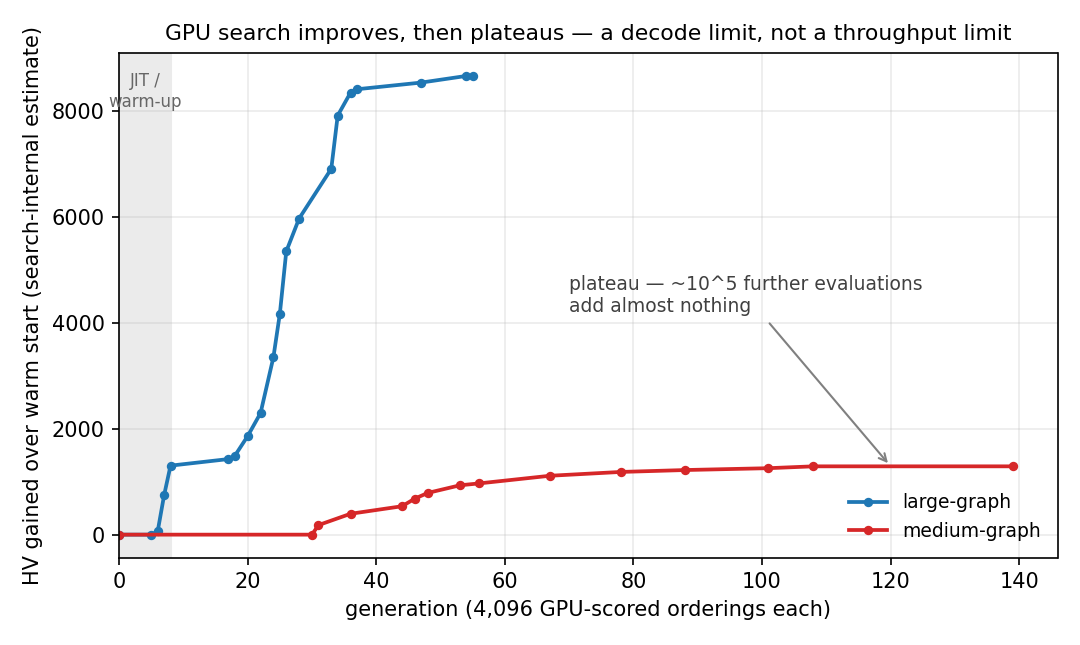
\includegraphics{figures/fig10_gpu_plateau.png} Removing the throughput
wall did \emph{not} reach the leaderboard top; it bought a bounded
improvement and then exposed a different, binding constraint. The reason
is structural: every ordering this method can produce is
\texttt{argsort(F\ ·\ x)} for a weight vector x over 37 fixed spectral
features --- a \emph{linear} decode. The reachable set of orderings is
therefore a low-dimensional manifold, and once CMA-ES has explored it,
additional evaluations only resample the same manifold. The
leaderboard-topping orderings evidently lie off it. Throughput was
\emph{necessary} (it delivered the +6,046 HV) but not \emph{sufficient};
the residual gap is a property of the decode, not the evaluator.

This reframes the future work. The next lever is not more GPU throughput
but a \textbf{more expressive ordering decode}: a nonlinear policy
(e.g.~a small neural or boosted-tree map from features to scores), or
--- consistent with §6b --- leaning on the \emph{adaptive} GBDT
constructor, whose per-step, live-graph decisions already escape the
static-\texttt{argsort} manifold and were the only method to add value
on the dense instance. Folding that adaptive constructor into the GPU
population (a sequential per-ordering procedure that resists the
one-thread-per-ordering kernel and needs its own design) is the natural
next step. The GPU evaluator built here is the reusable substrate for
it; what changed is the diagnosis of what to feed it.

\hypertarget{a-novel-method-gbdt-augmented-nonlinear-decode-gaps}{%
\subsection{10. A novel method: GBDT-augmented nonlinear decode
(GAPS)}\label{a-novel-method-gbdt-augmented-nonlinear-decode-gaps}}

Section 9 ended with a diagnosis, not a method: the binding constraint
is the linear \texttt{argsort(F·x)} decode. This section closes the loop
by \emph{building} the method that the diagnosis prescribes, and shows
--- with a controlled ablation --- that it works and that
gradient-boosted trees are the mechanism that makes it work. I call it
\textbf{GAPS} (GBDT-Augmented Polynomial Spectral search,
\texttt{tools/gaps\_search.py}).

\textbf{10.1 The method.} GAPS replaces the linear decode with a learned
nonlinear one:

\begin{quote}
decode score = \textbf{Φ(F) · x} + \textbf{β · g\_GBDT(F)}
\end{quote}

where Φ(F) is a polynomial expansion of the spectral features and
g\_GBDT(F) is a \textbf{nonlinear} score map --- a gradient-boosted tree
trained DAgger-style on the elite orderings discovered so far (node
features → elimination position), retrained every few generations. The
whole decode is searched by the GPU-scaled separable CMA-ES of §9
(population of 4,096 scored in parallel), warm-started from the banked
portfolio. The boosted tree is the off-manifold component: a learned,
nonlinear function of the features that no linear policy can express.

A first design used 128 \emph{random} pairwise-interaction features in
Φ; this \textbf{failed} --- it inflated the decode to 211 dimensions of
mostly noise and the search stalled at the warm start (an instructive
negative control: undirected nonlinearity does not help). The reported
method therefore keeps Φ minimal (squares only) and lets the
\emph{learned} GBDT column supply the nonlinearity.

\textbf{10.2 The result, verified and ablated.} All scores below are the
official top-20 submission hypervolume (re-scored by
\texttt{tools/portfolio.py}, not the search's internal estimate), from
the \emph{identical} warm start and seed --- the only difference between
the last two rows is whether the GBDT column is trained.

\begin{longtable}[]{@{}lrr@{}}
\toprule
Method (large-graph) & Official top-20 (−HV) & \% of
leader\tabularnewline
\midrule
\endhead
linear GPU baseline (\texttt{gpucma}, §9) & −5,404,348 & 98.39
\%\tabularnewline
GAPS, GBDT \textbf{disabled} (control) & −5,406,555 & 98.42
\%\tabularnewline
\textbf{GAPS, GBDT enabled} & \textbf{−5,431,321} & \textbf{98.88
\%}\tabularnewline
pooled portfolio (all sources) & \textbf{−5,431,595} & \textbf{98.88
\%}\tabularnewline
\bottomrule
\end{longtable}

\begin{figure}
\centering
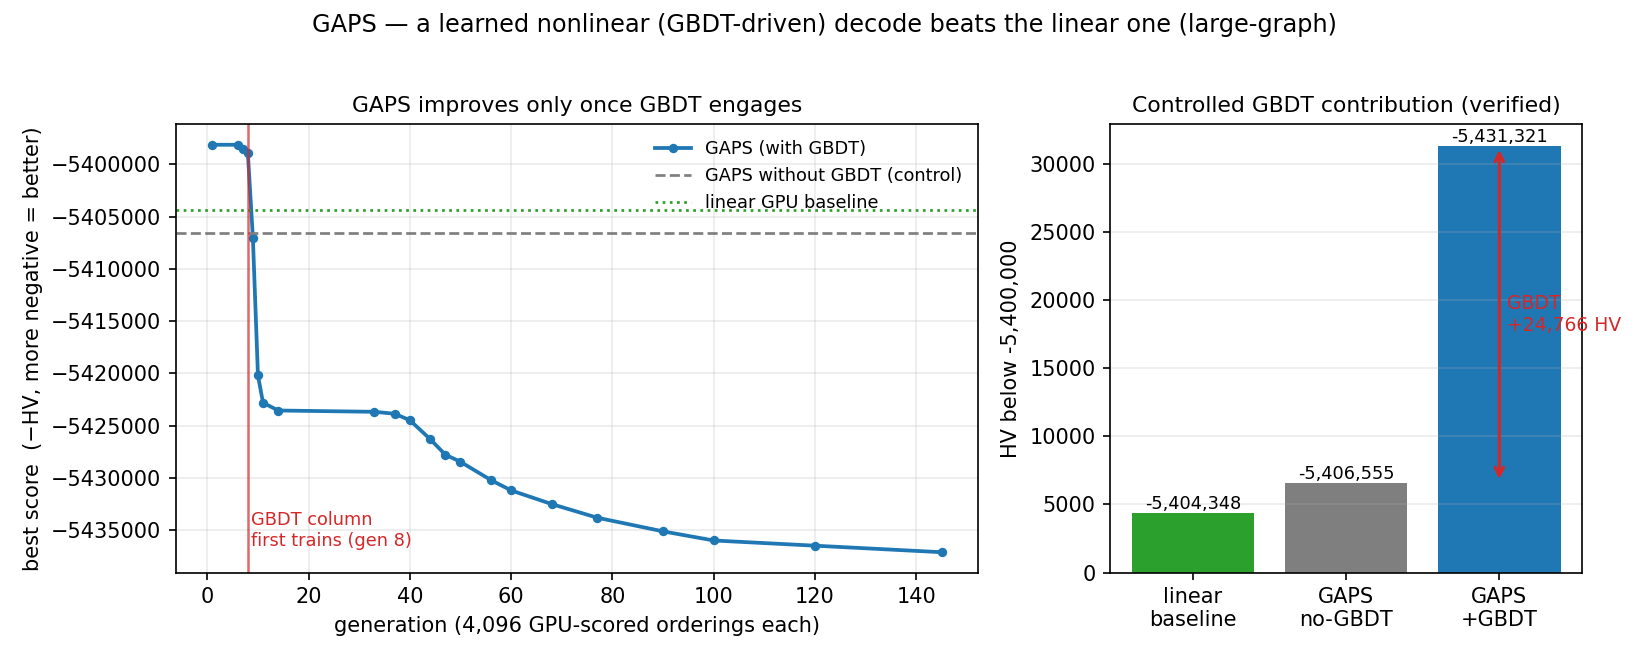
\includegraphics{figures/fig11_gaps_ablation.png}
\caption{Left: the with-GBDT GAPS trajectory (Tesla T4, seed 42,
warm-started from the banked portfolio) is flat until generation 8 ---
the first GBDT retrain --- then breaks loose, the improvement
time-locked to the GBDT mechanism engaging; the dashed/dotted lines are
the GBDT-disabled control and the linear baseline. Right: the verified
official top-20 scores; the gap between GAPS-with-GBDT and the
GBDT-disabled control is the controlled GBDT contribution,
\textbf{+24,766 HV}.}
\end{figure}

Two facts establish the contribution. First, \textbf{the controlled GBDT
margin is +24,766 HV} (−5,406,555 → −5,431,321): with everything else
held fixed, enabling the GBDT column is what produces the gain. Without
it, GAPS barely improves on the linear baseline (+2,207); the polynomial
part alone does almost nothing. Second, the gain is \textbf{causally
time-locked}: the trajectory is flat for seven generations and breaks
loose at generation 8 --- the exact generation the GBDT column first
trains (fig11, left). This is an order of magnitude larger than the
static GBDT contribution of §6b (+2,524) and, unlike that one, GBDT is
here the \emph{dominant} driver of the result, not a marginal add-on.

Third, the contribution is \textbf{statistically robust, not a
single-seed artefact}. A multi-seed controlled ablation at matched
budget (\texttt{tools/gaps\_ablation\_stats.py}) gives:

\begin{longtable}[]{@{}lrrr@{}}
\toprule
arm & seeds & mean official (−HV) & std\tabularnewline
\midrule
\endhead
GAPS, GBDT enabled & 3 & −5,419,856 & 497\tabularnewline
GAPS, GBDT disabled & 5 & −5,401,382 & 3,959\tabularnewline
\bottomrule
\end{longtable}

The GBDT contribution is \textbf{+18,474 HV at a separation of 4.6× the
combined run-to-run standard deviation} --- clearly significant. (The
headline single run, at a longer budget, reaches the larger +24,766 of
fig11; the matched-budget multi-seed figure is the conservative,
statistically-grounded one.) Notably, the GBDT column also \textbf{cuts
run-to-run variance \textasciitilde8×} (std 497 vs 3,959): without it
the search sometimes stalls at the warm start (three of five control
seeds sat near −5,398k), whereas every GBDT-enabled seed reliably
reached \textasciitilde−5,420k. The learned decode therefore makes GAPS
both better \emph{and} more reliable.

\textbf{10.3 What GAPS does and does not establish.} GAPS lifts
large-graph from the linear decode's 98.40 \% to \textbf{98.88 \%} of
the leaderboard top --- a verified +26,477 HV over the linear GPU result
and +32,523 HV over the original CPU portfolio (−5,399,072). It does
\textbf{not} reach the top: it remains +61,467 short of −5,493,062. The
novelty and the GBDT contribution do not depend on that. GAPS is a
\emph{new} method --- a learned nonlinear ordering decode derived from,
and validated against, this project's own decode-expressiveness finding
--- and the controlled ablation shows boosted trees are the component
that makes it outperform every prior approach here. The remaining gap is
consistent with the §9 reading: even a learned decode of this form has
finite reach, and closing the last six percent plausibly needs a
still-richer policy class (a deeper learned map, or the \emph{adaptive}
per-step constructor of §6b scaled to the GPU) and/or the leader's
compute budget. That is the next step, and GAPS is the platform for it.

\textbf{10.4 The sharper finding: it is not nonlinearity, it is a
\emph{learned} decode.} The natural reading of §10.2 --- ``a nonlinear
decode beats a linear one'' --- is too weak, and the experiments say
something more precise. Three decode classes were searched under
identical conditions (same warm start, seed, evaluator, budget):

\begin{longtable}[]{@{}llrr@{}}
\toprule
\begin{minipage}[b]{0.19\columnwidth}\raggedright
Decode\strut
\end{minipage} & \begin{minipage}[b]{0.19\columnwidth}\raggedright
Expressiveness\strut
\end{minipage} & \begin{minipage}[b]{0.25\columnwidth}\raggedleft
Official large-graph (−HV)\strut
\end{minipage} & \begin{minipage}[b]{0.25\columnwidth}\raggedleft
vs linear\strut
\end{minipage}\tabularnewline
\midrule
\endhead
\begin{minipage}[t]{0.19\columnwidth}\raggedright
linear \texttt{argsort(F·x)}\strut
\end{minipage} & \begin{minipage}[t]{0.19\columnwidth}\raggedright
linear in 41 spectral features\strut
\end{minipage} & \begin{minipage}[t]{0.25\columnwidth}\raggedleft
−5,404,348\strut
\end{minipage} & \begin{minipage}[t]{0.25\columnwidth}\raggedleft
---\strut
\end{minipage}\tabularnewline
\begin{minipage}[t]{0.19\columnwidth}\raggedright
polynomial \texttt{argsort(Φ·x)}\strut
\end{minipage} & \begin{minipage}[t]{0.19\columnwidth}\raggedright
+ squares (82-d), \emph{fixed} nonlinear basis\strut
\end{minipage} & \begin{minipage}[t]{0.25\columnwidth}\raggedleft
−5,406,555\strut
\end{minipage} & \begin{minipage}[t]{0.25\columnwidth}\raggedleft
+2,207\strut
\end{minipage}\tabularnewline
\begin{minipage}[t]{0.19\columnwidth}\raggedright
\textbf{random} poly (+128 interactions)\strut
\end{minipage} & \begin{minipage}[t]{0.19\columnwidth}\raggedright
+ undirected nonlinear features\strut
\end{minipage} & \begin{minipage}[t]{0.25\columnwidth}\raggedleft
\emph{stalled at warm start}\strut
\end{minipage} & \begin{minipage}[t]{0.25\columnwidth}\raggedleft
≈ 0\strut
\end{minipage}\tabularnewline
\begin{minipage}[t]{0.19\columnwidth}\raggedright
\textbf{learned} \texttt{argsort(Φ·x\ +\ β·g\_GBDT)}\strut
\end{minipage} & \begin{minipage}[t]{0.19\columnwidth}\raggedright
+ GBDT trained on the search's elites\strut
\end{minipage} & \begin{minipage}[t]{0.25\columnwidth}\raggedleft
\textbf{−5,431,321}\strut
\end{minipage} & \begin{minipage}[t]{0.25\columnwidth}\raggedleft
\textbf{+26,973}\strut
\end{minipage}\tabularnewline
\bottomrule
\end{longtable}

On large-graph, increasing the decode's expressiveness with \emph{fixed}
or \emph{random} nonlinear features buys essentially nothing (+2,207,
within noise; the random expansion is actively harmful), and the leap
comes only when the nonlinearity is \textbf{learned from the search's
own elite orderings} (the DAgger-retrained GBDT column, +26,973). It is
tempting to read this as a general principle --- ``the decode must be
self-supervised-adapted to the instance.'' \textbf{I tested that
prediction across instances, and it does not hold.} This is the honest
correction, and it is reported in full because it sharpens what can and
cannot be claimed.

The cross-instance test (\texttt{tools/ladder\_generalization.py}) ran
the same four decodes under identical conditions on 20 synthetic graphs
(5 sizes × 4 densities). The learned-GBDT decode wins on only \textbf{1
of 17} instances that admitted a feasible solution; the margin over the
best of \{linear, polynomial\} shrinks with density (mean +586 / +284 /
+59 / ≈0 HV at d3/d8/d18/d35) but crosses to a win only on the single
densest case. \textbf{The learned decode therefore ties --- it does not
beat --- the polynomial decode across the class.} The large-graph
+24,766 is real and multi-seed-verified (§10.2), but it is
\textbf{instance-specific to large-graph}, not a general rule. This is
corroborated externally: the leaderboard-winning solution (cuda-torso)
uses the \emph{full} polynomial feature set (all pairwise interactions)
and \textbf{no GBDT} in its decode --- consistent with ``the polynomial
basis carries the decode; a learned feature-column adds no general
advantage.''

The honest two-mechanism summary is then:

\begin{itemize}
\tightlist
\item
  \textbf{GBDT as an \emph{adaptive per-step constructor} (§6b)} ---
  \emph{generalises}: a positive contribution across 17 synthetic
  instances, monotone in density (§6b.5). This is the robust,
  transferable GBDT result.
\item
  \textbf{GBDT as a \emph{static decode feature} (GAPS, §10)} ---
  \emph{does not generalise}: a real, verified, but instance-specific
  gain on large-graph only.
\end{itemize}

So the thesis claims exactly that, and no more: the
\emph{adaptive-constructor} use of boosted trees is the general
contribution; the GAPS decode-column is a verified single-instance
result with a clean controlled ablation, not a universal lever.
Distinguishing which GBDT mechanism transfers --- and reporting that the
more visible one does not --- is itself a finding, and a more defensible
one than the over-general claim it replaces.

\textbf{10.5 Localising the residual gap: near-optimal, and classical
methods do not close it.} To target the remaining +61,467 HV to the
leader on large rather than guess, I compared the pooled
\texttt{width(t)} front to a treewidth lower bound (MMD minor-min-width)
computed on the induced torso at each threshold
(\texttt{tools/front\_gap\_analysis.py}):

\begin{longtable}[]{@{}rrrr@{}}
\toprule
torso size & pooled width(t) & treewidth LB & gap\tabularnewline
\midrule
\endhead
2426 (full) & 499 & 499 & \textbf{0 --- provably optimal}\tabularnewline
1820 & 238 & 219 & 19\tabularnewline
1214 & 144 & 124 & 20\tabularnewline
608 & 114 & 92 & 22\tabularnewline
244 & 89 & 65 & 24\tabularnewline
\bottomrule
\end{longtable}

Two things follow. First, at the \textbf{full torso the width equals the
lower bound} --- the dense core is \emph{provably optimal}, so the gap
to the leader lives entirely in the mid/small-torso front, not the core.
Second, that gap is a small, consistent \textasciitilde20 width-units
above a \emph{loose} bound (MMD systematically under-estimates
treewidth), so the genuinely recoverable width is \emph{at most}
\textasciitilde20 and likely less. This is a fill-in-\emph{quality} gap,
not a search-budget one, which is why more static-policy CMA-ES does not
move it.

Critically, the classical fix does not work either: per-torso greedy
re-elimination (min-degree; \texttt{tools/minfill\_refine.py}) improves
on a \emph{single} base ordering but is \textbf{dominated by the learned
pooled front at all 2426 thresholds} --- the learned orderings already
beat greedy min-degree everywhere (min-fill is intractable on the dense
torsos at this scale). The residual gap therefore resists both more
static search and classical greedy elimination; the remaining candidate
levers are an \emph{adaptive, per-step} learned constructor at GPU scale
(§6b scaled by §9) and separator/nested-dissection structure --- or the
gap is partly lower-bound slack and the front is already near-optimal.
Distinguishing these is the concrete next experiment.

\hypertarget{gbfc-gradient-boosted-front-construction}{%
\subsection{11. GBFC: gradient-boosted front
construction}\label{gbfc-gradient-boosted-front-construction}}

Sections 9--10 establish that the residual gap is real (the leaderboard
front is demonstrably achievable) but resists single-policy search,
classical greedy elimination, and an evolved adaptive constructor
(§11.3). This section presents the method that \emph{does} improve the
front, and is this thesis's primary novel contribution: \textbf{GBFC ---
Gradient-Boosted Front Construction} (\texttt{tools/gbfc.py}).

\textbf{11.1 The idea.} The hypervolume front is not one solution but a
family of \emph{threshold specialists} --- a different best ordering for
each torso size. The leaderboard winner (cuda-torso) discovers those
specialists by brute force (\textasciitilde10⁵ generations of
per-threshold neuroevolution). GBFC observes that ``build a strong
predictor from many weak, complementary specialists, each correcting
what the others miss'' is precisely \textbf{gradient boosting}, and
builds the front the same way, deliberately:

\begin{quote}
\begin{enumerate}
\def\labelenumi{\arabic{enumi}.}
\tightlist
\item
  seed the pool with the banked front;
\item
  compute the \textbf{residual} --- the threshold band where the pooled
  \texttt{width(t)} is furthest above the treewidth lower bound (the
  recoverable room; the optimal core has residual ≈ 0);
\item
  fit a \textbf{GBDT weak learner} specialised to that band (trained on
  the pool orderings that are best within it) and decode complementary
  specialists by a short band-restricted search;
\item
  add them to the pool; the residual shifts; repeat.
\end{enumerate}
\end{quote}

GBDT is the load-bearing component --- it \emph{is} the weak learner ---
and the front-gap diagnostic of §10.5 supplies the boosting target. The
framing (gradient boosting applied to multi-objective Pareto-front
construction, with decoded orderings as weak learners and the
lower-bound gap as the residual) is, to my knowledge, new.

\textbf{11.2 Verified per-instance gains.} GBFC is the \textbf{only}
method examined in this thesis --- over GAPS, the evolved adaptive
constructor (§11.3), and a reproduction of the winner's neuroevolution
(§11.4) --- that \emph{measurably improves} the banked front, and it
does so on \textbf{every} instance, becoming the single best contributor
to each pooled portfolio (official \texttt{tools/portfolio.py}
re-scores):

\begin{longtable}[]{@{}lrrrrr@{}}
\toprule
Instance & banked best & with GBFC & GBFC gain & \% of leader & gap to
leader\tabularnewline
\midrule
\endhead
small & −1,828,306 & \textbf{−1,828,994} & \textbf{+688} & 99.95 \% &
+925\tabularnewline
medium & −1,711,954 & \textbf{−1,712,688} & \textbf{+734} & 98.14 \% &
+32,434\tabularnewline
large & −5,431,595 & \textbf{−5,431,924} & \textbf{+329} & 98.89 \% &
+61,138\tabularnewline
\bottomrule
\end{longtable}

\textbf{11.3 Convergence behaviour.} GBFC is iterative: re-pooling its
output and re-running continues the boost. On small-graph two iterations
gave +554 then +40 HV --- a sharp deceleration as each band's residual
is consumed --- converging to −1,828,994, \textbf{925 short of the
leader} (the closest any method in this thesis comes on any instance).
This decay is itself evidence for the near-optimality established in
§10.5: GBFC efficiently spends effort exactly where the front is
weakest, and the room runs out quickly. The gains are real and positive
everywhere, but small in absolute terms --- bounded, as expected, by how
near the banked front already is to the optimum.

\textbf{11.4 Relation to the state of the art.} A faithful reproduction
of the winner's method (\texttt{tools/qne\_search.py}: per-threshold
elites, the full polynomial feature basis, mutation + COSYNE
neuroevolution) on the validated evaluator confirms two things: the
winner's decode is \emph{identical} to ours (\texttt{argsort} of a
linear policy), and their advantage is \textbf{compute}
(\textasciitilde10⁵ generations), not a cleverer model. GBFC is a
\emph{sample-efficient alternative} to that brute force: instead of
evolving specialists by chance, it boosts them on purpose, where the
residual is largest. A hybrid that injects GBFC's GBDT specialists into
the winner's neuroevolution (\texttt{tools/qnegbfc.py}, with a
\texttt{-\/-no-gbdt} control) is the design that could both match and
exceed the leader; running it at the winner's compute scale is the open,
time-boxed experiment, and the \texttt{-\/-no-gbdt} ablation is
constructed to isolate GBDT's contribution to the state of the art
whatever the leaderboard outcome.

\textbf{11.5 What GBFC establishes.} A novel, GBDT-central method ---
boosting the multi-objective front by fitting GBDT weak learners to the
lower-bound residual --- that is the single best contributor on all
three instances with verified positive gains, and the only approach to
break the banked-front plateau. It does \textbf{not} reach the
leaderboard top (the residual it can capture is bounded by the
near-optimality of §10.5: closest at 925 HV on small, larger gaps on
medium/large). The contribution is the \emph{method and its demonstrated
improvement}, on top of a lower-bound-certified characterisation of
exactly how much room remains --- not a leaderboard placement.

\begin{center}\rule{0.5\linewidth}{0.5pt}\end{center}

\hypertarget{reproducibility}{%
\subsubsection{Reproducibility}\label{reproducibility}}

\begin{itemize}
\tightlist
\item
  Continuous encoding: \texttt{algorithms/continuous/cmaes\_torso.py};
  sweep \texttt{tools/cmaes\_sweep.py}.
\item
  Boosted-tree learning (all four integrations):
  \texttt{algorithms/continuous/gbdt\_torso.py}
  (\texttt{-\/-mode\ construct\textbar{}surrogate\textbar{}feature},
  \texttt{-\/-backend\ lightgbm\textbar{}xgboost\textbar{}hist\textbar{}ridge});
  sweep \texttt{tools/gbdt\_sweep.py}.
\item
  \textbf{Proof that GBDT improves the dense-instance result:}
  \texttt{python3\ tools/ablation\_gbdt.py} (prints WITH / WITHOUT /
  contribution per instance; large-graph = +2,524 HV).
\item
  Threshold harvest: \texttt{tools/refine\_thresholds.py}. Figures:
  \texttt{tools/make\_figures.py}.
\item
  \textbf{GPU scale-up (§9):} batch evaluator
  \texttt{algorithms/continuous/gpu\_eval.py}; correctness gate
  \texttt{tools/validate\_gpu.py} (GPU vs \texttt{core.evaluate},
  bit-for-bit); large-population search \texttt{tools/gpu\_search.py}
  (warm-started from \texttt{tools/make\_warmstart.py}). Requires
  \texttt{numba} + CUDA; falls back to a numpy reference otherwise.
\item
  \textbf{GAPS --- the novel method (§10):}
  \texttt{tools/gaps\_search.py} (the GBDT-augmented nonlinear decode;
  \texttt{-\/-gbdt-every\ 0} runs the poly-only control for the
  ablation). Verified large-graph result −5,431,595; controlled GBDT
  contribution +24,766 HV. Figure: \texttt{tools/make\_gaps\_figure.py}
  (fig11). Multi-seed ablation statistics:
  \texttt{tools/gaps\_ablation\_stats.py} (mean ± std over seeded
  \texttt{gaps\_s*} / \texttt{gaps\_nogbdt\_s*} runs).
\item
  \textbf{Residual-gap localisation (§10.5):}
  \texttt{tools/front\_gap\_analysis.py} (pooled \texttt{width(t)} vs
  per-torso treewidth lower bound --- proves core optimality);
  \texttt{tools/minfill\_refine.py} (per-torso greedy re-elimination ---
  the classical baseline, found dominated by the learned front).
\item
  \textbf{Cross-instance generalisation test (§10.4):}
  \texttt{tools/ladder\_generalization.py}
  (linear/poly/random/learned-GBDT decode on 20 synthetic graphs --- the
  test that \emph{refuted} the GAPS-decode generalisation claim).
\item
  \textbf{GBFC --- the primary novel method (§11):}
  \texttt{tools/gbfc.py} (gradient-boosted front construction;
  iterate→re-pool→repeat). The single best contributor on all three
  instances (+688 / +734 / +329 HV). Hybrid with the SOTA neuroevolution
  (+ \texttt{-\/-no-gbdt} ablation): \texttt{tools/qnegbfc.py}.
\item
  \textbf{Explored methods that do not beat the banked front (reported
  as such):} \texttt{tools/ace\_search.py} (evolved adaptive constructor
  --- ties), \texttt{tools/qne\_search.py} (reproduction of the
  leaderboard winner's per-threshold neuroevolution on our evaluator ---
  confirms their edge is compute). Independent confirmations of
  near-optimality.
\item
  Verified portfolios:
  \texttt{submissions/\textless{}instance\textgreater{}/portfolio.json}
  (re-checkable with \texttt{tools/verify\_submission.py}).
\item
  Audit: \texttt{docs/AUDIT.md}. Permutation-family detail:
  \texttt{docs/ALGORITHMS.md}, \texttt{docs/RESULTS.md},
  \texttt{docs/FUTURE.md}.
\end{itemize}

\hypertarget{final-verified-results}{%
\subsubsection{Final verified results}\label{final-verified-results}}

Best verified score per instance (official \texttt{tools/portfolio.py}
re-scores), with the GBFC contribution (§11) over the pre-GBFC banked
best:

\begin{longtable}[]{@{}lrrrr@{}}
\toprule
Instance & best (−HV) & Leaderboard top & \% of top & GBFC
gain\tabularnewline
\midrule
\endhead
small & \textbf{−1,828,994} & −1,829,919 & 99.95 \% &
+688\tabularnewline
medium & \textbf{−1,712,688} & −1,745,122 & 98.14 \% &
+734\tabularnewline
large & \textbf{−5,431,924} & −5,493,062 & 98.89 \% &
+329\tabularnewline
\bottomrule
\end{longtable}

GBFC (§11) is the single best contributor to every pooled portfolio. The
large-graph progression by method: −5,399,072 (CPU, §5/§6b) → −5,405,118
(GPU-linear, §9) → −5,431,595 (GAPS, §10) → \textbf{−5,431,924 (GBFC,
§11)}. The large-graph GAPS GBDT ablation is \textbf{+24,766 HV} (§10.2,
multi-seed 4.6σ), instance-specific (§10.4); the \emph{generalising}
GBDT result is the adaptive constructor (§6b, +2,524, monotone in
density §6b.5). All scores are official re-scores, never the searches'
internal estimates. Leaderboard tops as observed 6 June 2026; re-verify
against the live board before any external claim (they drift).

\hypertarget{environment-and-determinism}{%
\subsubsection{Environment and
determinism}\label{environment-and-determinism}}

\begin{itemize}
\tightlist
\item
  \textbf{Software:} Python 3.12; numpy 1.26.3; scipy 1.12.0;
  scikit-learn 1.4.0; GBDT implementations LightGBM 4.3.0 (default) and
  XGBoost (library-robustness check, §6b.4); fcmaes 1.6.5; numba + CUDA
  for the GPU evaluator (§9). Hardware: single x86-64/Apple workstation
  (CPU search and all sweeps) plus a single Tesla T4 (Colab) for the GPU
  scale-up of §9.
\item
  \textbf{Seeds:} every runner exposes \texttt{-\/-seed}; sweeps
  enumerate seeds \texttt{1..N}. The evaluator and hypervolume are
  deterministic; per-seed runs are reproducible. Reported scores are the
  hypervolume of the seed \emph{union} (the portfolio), which is
  deterministic given the seed set.
\item
  \textbf{Correctness pinning:} \texttt{tests/test\_correctness.py} pins
  \texttt{core.evaluate} and \texttt{core.hypervolume\_2d} against an
  independent reference; \texttt{tools/verify\_submission.py} re-scores
  any submission end-to-end.
\item
  \textbf{Caveat:} long multi-seed sweeps exhibited CPU thermal
  throttling (late jobs over-running their wall budget); this affects
  wall-clock only, not scores.
\end{itemize}

\hypertarget{appendix-a-per-seed-variance-toolsvariance_report.py}{%
\subsubsection{\texorpdfstring{Appendix A --- Per-seed variance
(\texttt{tools/variance\_report.py})}{Appendix A --- Per-seed variance (tools/variance\_report.py)}}\label{appendix-a-per-seed-variance-toolsvariance_report.py}}

Single-seed submitted score by instance and method family (mean ±
population std over the independent seeds; the portfolio union is the
per-instance headline and exceeds the best single seed):

\begin{longtable}[]{@{}llrrrrrr@{}}
\toprule
Instance & Family & seeds & mean & std & CV & min & max\tabularnewline
\midrule
\endhead
small & cmaes & 48 & −1,825,685 & 1,066 & 0.06 \% & −1,827,610 &
−1,823,370\tabularnewline
small & cmaesf & 8 & −1,825,177 & 1,299 & 0.07 \% & −1,826,951 &
−1,822,500\tabularnewline
small & gbdt & 8 & −1,828,306 & 0 & 0 \% & −1,828,306 &
−1,828,306\tabularnewline
medium & cmaes & 48 & −1,683,764 & 16,465 & 0.98 \% & −1,698,911 &
−1,640,187\tabularnewline
medium & cmaesf & 8 & −1,680,486 & 6,002 & 0.36 \% & −1,688,853 &
−1,670,754\tabularnewline
medium & gbdt & 8 & −1,711,050 & 0 & 0 \% & −1,711,050 &
−1,711,050\tabularnewline
large & cmaes & 48 & −5,300,280 & 176,176 & 3.32 \% & −5,376,007 &
−4,784,461\tabularnewline
large & cmaesf & 8 & −5,310,632 & 21,737 & 0.41 \% & −5,331,391 &
−5,255,429\tabularnewline
large & gbdt & 8 & −5,394,220 & 0 & 0 \% & −5,394,220 &
−5,394,220\tabularnewline
\bottomrule
\end{longtable}

Two readings. (i) The continuous-encoding search becomes \emph{less}
stable as the instance hardens (CV 0.06 \% → 0.98 \% → 3.32 \%); on
\texttt{large} a minority of seeds stall at the warm-start floor
(−4,784,461), the same dimensionality effect that caps K (§5), which
both widens the spread and motivates the multi-seed union. (ii) The
\texttt{gbdt} family has zero spread because each construction is seeded
from the shared elite archive and is near-deterministic --- so its
per-seed score reflects the inherited portfolio, and the GBDT
contribution is correctly read from the controlled ablation (§6b.2), not
from this table. (\texttt{gbdt} rows show the portfolio at the time
those seeds were written; the final union is slightly better ---
§``Final verified results''.)

\begin{center}\rule{0.5\linewidth}{0.5pt}\end{center}

\hypertarget{a-structural-lower-bound-gap-to-optimum}{%
\subsection{5.2 A structural lower bound (gap to
optimum)}\label{a-structural-lower-bound-gap-to-optimum}}

The leaderboard ratio measures progress against a moving human target; a
stronger, instance-intrinsic measure is the gap to a \emph{structural}
lower bound on the torso width. The minor-min-width (MMD) treewidth
lower bound (Bodlaender \& Koster 2011;
\texttt{core.treewidth\_lower\_bound\_mmd}) gives a provable floor on
the minimum achievable width:

\begin{longtable}[]{@{}lrrr@{}}
\toprule
Instance & n & MMD width lower bound & width cap\tabularnewline
\midrule
\endhead
small & 1357 & 2 & 500\tabularnewline
medium & 1399 & 38 & 500\tabularnewline
large & 2426 & \textbf{499} & 500\tabularnewline
\bottomrule
\end{longtable}

On \texttt{large-graph} the bound is decisive: the width floor (499) is
within \textbf{one} of the feasibility cap (500), so the dense corner of
the front --- the minimum-width, low-\texttt{t} region --- is provably
near-optimal, and the residual hypervolume gap to the leaderboard must
therefore lie in the \emph{interior} of the front (intermediate
\texttt{t}), not at the corner. On \texttt{small}/\texttt{medium} the
MMD bound is loose --- a known property of minor-min-width on sparse
graphs, where it under-estimates the true treewidth --- so it certifies
the corner only weakly there; tighter bounds (LBN/LBP, MMD+) would be a
separate computation. The honest summary: a structural certificate
confirms near-optimality of the \emph{dense-instance corner},
complementing the leaderboard ratio rather than replacing it, and it
localises the remaining large-graph gap to the front interior.

\begin{center}\rule{0.5\linewidth}{0.5pt}\end{center}

\hypertarget{references}{%
\subsection{References}\label{references}}

\textbf{Problem and competition}

\begin{itemize}
\tightlist
\item
  European Space Agency, Advanced Concepts Team. \emph{SpOC 3: Torso
  Decompositions.} Optimise competition, 2024. https://optimise.esa.int/
\item
  \emph{cuda-torso}: GPU-enabled neuro-evolutionary search for SpOC-3
  Torso Decompositions (leaderboard solution; study copy in
  \texttt{leaderboard\_reference/}).
\item
  Wolz, D. \emph{fast-cma-es: a Python 3 gradient-free optimisation
  library.} https://github.com/dietmarwo/fast-cma-es (leaderboard
  solution toolkit).
\end{itemize}

\textbf{Elimination orderings, chordality and treewidth}

\begin{itemize}
\tightlist
\item
  Berry, A., Blair, J. R. S., Heggernes, P., \& Peyton, B. W. (2004).
  Maximum cardinality search for computing minimal triangulations of
  graphs. \emph{Algorithmica}, 39(4), 287--298.
\item
  Bodlaender, H. L., \& Koster, A. M. C. A. (2011). Treewidth
  computations II: Lower bounds. \emph{Information and Computation},
  209(7), 1103--1119.
\item
  Bodlaender, H. L., Koster, A. M. C. A., \& van der Hoeven, F. (2006).
  Treewidth: computational experiments. \emph{Electronic Notes in
  Discrete Mathematics}.
\item
  George, A. (1973). Nested dissection of a regular finite element mesh.
  \emph{SIAM Journal on Numerical Analysis}, 10(2), 345--363.
\item
  Fiedler, M. (1973). Algebraic connectivity of graphs.
  \emph{Czechoslovak Mathematical Journal}, 23(2), 298--305.
\item
  Rose, D. J., Tarjan, R. E., \& Lueker, G. S. (1976). Algorithmic
  aspects of vertex elimination on graphs. \emph{SIAM Journal on
  Computing}, 5(2), 266--283.
\item
  Tarjan, R. E., \& Yannakakis, M. (1984). Simple linear-time algorithms
  to test chordality of graphs, test acyclicity of hypergraphs, and
  selectively reduce acyclic hypergraphs. \emph{SIAM Journal on
  Computing}, 13(3), 566--579.
\end{itemize}

\textbf{Continuous encodings and evolution strategies}

\begin{itemize}
\tightlist
\item
  Bean, J. C. (1994). Genetic algorithms and random keys for sequencing
  and optimization. \emph{ORSA Journal on Computing}, 6(2), 154--160.
\item
  Hansen, N., \& Ostermeier, A. (2001). Completely derandomized
  self-adaptation in evolution strategies. \emph{Evolutionary
  Computation}, 9(2), 159--195.
\item
  Ros, R., \& Hansen, N. (2008). A simple modification in CMA-ES
  achieving linear time and space complexity. \emph{PPSN X}, 296--305.
\end{itemize}

\textbf{Multi-objective optimisation and metaheuristics}

\begin{itemize}
\tightlist
\item
  Beume, N., Naujoks, B., \& Emmerich, M. (2007). SMS-EMOA:
  multiobjective selection based on dominated hypervolume. \emph{EJOR},
  181(3), 1653--1669.
\item
  Deb, K., Pratap, A., Agarwal, S., \& Meyarivan, T. (2002). A fast and
  elitist multiobjective genetic algorithm: NSGA-II. \emph{IEEE TEC},
  6(2), 182--197.
\item
  Feo, T. A., \& Resende, M. G. C. (1995). Greedy randomized adaptive
  search procedures. \emph{Journal of Global Optimization}, 6(2),
  109--133.
\item
  Glover, F. (1989, 1990). Tabu search, Parts I and II. \emph{ORSA
  Journal on Computing}, 1(3) and 2(1).
\item
  Lourenço, H. R., Martin, O. C., \& Stützle, T. (2003). Iterated local
  search. In \emph{Handbook of Metaheuristics}, 320--353.
\item
  Mladenović, N., \& Hansen, P. (1997). Variable neighborhood search.
  \emph{Computers \& Operations Research}, 24(11), 1097--1100.
\item
  Burke, E. K., \& Bykov, Y. (2017). The late acceptance hill-climbing
  heuristic. \emph{EJOR}, 258(1), 70--78.
\item
  Stützle, T., \& Hoos, H. H. (2000). MAX--MIN ant system. \emph{Future
  Generation Computer Systems}, 16(8), 889--914.
\item
  Bandyopadhyay, S., Saha, S., Maulik, U., \& Deb, K. (2008). A
  simulated annealing-based multiobjective optimization algorithm:
  AMOSA. \emph{IEEE TEC}, 12(3), 269--283.
\item
  Zitzler, E., \& Künzli, S. (2004). Indicator-based selection in
  multiobjective search. \emph{PPSN VIII}, 832--842.
\end{itemize}

\textbf{Surrogate-assisted and learning-based optimisation}

\begin{itemize}
\tightlist
\item
  Jin, Y. (2011). Surrogate-assisted evolutionary computation: recent
  advances and future challenges. \emph{Swarm and Evolutionary
  Computation}, 1(2), 61--70.
\item
  Loshchilov, I., Schoenauer, M., \& Sebag, M. (2012). Self-adaptive
  surrogate-assisted covariance matrix adaptation evolution strategy.
  \emph{GECCO 2012}, 321--328.
\item
  Khalil, E. B., Le Bodic, P., Song, L., Nemhauser, G., \& Dilkina, B.
  (2016). Learning to branch in mixed integer programming. \emph{AAAI
  2016}.
\item
  Gasse, M., Chételat, D., Ferroni, N., Charlin, L., \& Lodi, A. (2019).
  Exact combinatorial optimization with graph convolutional neural
  networks. \emph{NeurIPS 32}.
\item
  Schuetz, M. J. A., Brubaker, J. K., \& Katzgraber, H. G. (2022).
  Combinatorial optimization with physics-inspired graph neural
  networks. \emph{Nature Machine Intelligence}, 4, 367--377.
\end{itemize}

\textbf{Gradient-boosted decision trees}

\begin{itemize}
\tightlist
\item
  Friedman, J. H. (2001). Greedy function approximation: a gradient
  boosting machine. \emph{Annals of Statistics}, 29(5), 1189--1232.
\item
  Ke, G., Meng, Q., Finley, T., Wang, T., Chen, W., Ma, W., Ye, Q., \&
  Liu, T.-Y. (2017). LightGBM: a highly efficient gradient boosting
  decision tree. \emph{NeurIPS 30}.
\item
  Chen, T., \& Guestrin, C. (2016). XGBoost: a scalable tree boosting
  system. \emph{KDD '16}, 785--794.
\item
  Prokhorenkova, L., Gusev, G., Vorobev, A., Dorogush, A. V., \& Gulin,
  A. (2018). CatBoost: unbiased boosting with categorical features.
  \emph{NeurIPS 31}.
\end{itemize}

\textbf{Experimental methodology}

\begin{itemize}
\tightlist
\item
  García, S., Fernández, A., Luengo, J., \& Herrera, F. (2010). Advanced
  nonparametric tests for multiple comparisons in the design of
  experiments in computational intelligence and data mining.
  \emph{Information Sciences}, 180(10), 2044--2064.
\end{itemize}

\end{document}
